% Created 2011-09-09 Fri 14:42
\documentclass[captions=tableheading]{scrbook}



\subtitle{Second Edition}

\usepackage{lmodern}
\renewcommand{\sfdefault}{lmss}
\renewcommand{\ttdefault}{lmtt}

% needed packages
\usepackage{amsmath}
\usepackage{amssymb}
\usepackage{amsthm}
\usepackage[english]{babel}
\usepackage{epsfig}
\usepackage{fancyvrb}
\usepackage{fixltx2e}
\usepackage{float}
%\usepackage{floatflt}
\usepackage[T1]{fontenc}
\usepackage{footnote}
%\usepackage{graphics}
\usepackage{graphicx}
\usepackage[utf8]{inputenc}
\usepackage{latexsym}
\usepackage{longtable}
\usepackage{makeidx}
\usepackage{marvosym}
\usepackage{multicol}
%\usepackage{pslatex}
%\usepackage{showidx}
\usepackage{soul}
\usepackage{srcltx}
\usepackage{stmaryrd}
\usepackage{subfig}
\usepackage{textcomp}
%\usepackage{theorem}
\usepackage[subfigure]{tocloft}
\usepackage{txfonts}
\usepackage{upgreek}
\usepackage{url}
\usepackage{varioref}
\usepackage{verbatim}
%\usepackage{wasysym}
\usepackage{wrapfig}


% Page setup
\usepackage[paperwidth=7.44in,paperheight=9.69in]{geometry}
\geometry{verbose,tmargin=1in,bmargin=1in,lmargin=1in,rmargin=1in}
\pagestyle{headings}
\setcounter{secnumdepth}{2}
\setcounter{tocdepth}{1}

\makeindex

% PDF settings
\usepackage[hyperref,x11names]{xcolor}
\usepackage[	unicode=true, 
		bookmarks=true, 
		bookmarksnumbered=true, 
		bookmarksopen=true, 
		bookmarksopenlevel=0, 
		breaklinks=true,
		pdfborder={0 0 0},
		backref=page,
		colorlinks=true]{hyperref}
\hypersetup{pdftitle={Introduction to Probability and Statistics Using R},
 		pdfauthor={G. Jay Kerns}, 
		linkcolor=Firebrick4, 
		citecolor=black, 
		urlcolor=SteelBlue4}

% Listings setup
\usepackage{color}
\usepackage{listings}
\lstset{basicstyle={\ttfamily},
	language=R,
	breaklines=true,
	breakatwhitespace=true,
	keywordstyle={\ttfamily},
	numberstyle = {\ttfamily},
	morestring=[b]"
}




%%%%%%%%%%%%%%%%%%%%%%%%%%%%%% LyX specific LaTeX commands.
\providecommand{\LyX}{L\kern-.1667em\lower.25em\hbox{Y}\kern-.125emX\@}
\newcommand{\noun}[1]{\textsc{#1}}
%% Because html converters don't know tabularnewline
\providecommand{\tabularnewline}{\\}

% special logos
\providecommand{\IPSUR}
{\textsc{I\kern 0ex\lower-0.3ex\hbox{\small P}\kern -0.5ex\lower0.4ex\hbox{\footnotesize S}\kern -0.25exU}\kern -0.1ex\lower 0.15ex\hbox{\textsf{\large R}}\@}

%  user defined commands
% special operators

\renewcommand{\vec}[1]{\mbox{\boldmath$#1$}}

\makeatletter

%%%%%%%%%%%%%%%%%%%%%%%%%%%%%% Textclass specific LaTeX commands.

\numberwithin{equation}{section}
\numberwithin{figure}{section}

\theoremstyle{plain}
  \newtheorem{thm}{Theorem}[chapter]
  \newtheorem{fact}[thm]{Fact}
  \newtheorem{ax}[thm]{Axiom}
  \newtheorem{prop}[thm]{Proposition}
  \newtheorem{cor}[thm]{Corollary}
  \newtheorem{assumption}[thm]{Assumption}

\theoremstyle{definition}
  \newtheorem{defn}[thm]{Definition}
  \newtheorem{example}[thm]{Example}
  \newtheorem{xca}{Exercise}[chapter]

\theoremstyle{remark}
  \newtheorem{note}[thm]{Note}
  \newtheorem{rem}[thm]{Remark}
  \newtheorem*{note*}{Note}

\setlength{\cftfignumwidth}{1.5cm}

\@ifundefined{showcaptionsetup}{}{%
 \PassOptionsToPackage{caption=false}{subfig}}
\usepackage{subfig}
\AtBeginDocument{
  \def\labelitemii{\(\circ\)}
}

\makeatother


\newenvironment{exampletoo}{\begin{example}}{\end{example}}


\providecommand{\alert}[1]{\textbf{#1}}

\title{Probability}
\author{G. Jay Kerns}
\date{\today}

\begin{document}

\maketitle

% Org-mode is exporting headings to 3 levels.

\chapter{Probability}
\label{sec-1}

\label{cha:Probability}


\noindent 
In this chapter we define the basic terminology associated with probability and derive some of its properties. We discuss three interpretations of probability. We discuss conditional probability and independent events, along with Bayes' Theorem. We finish the chapter with an introduction to random variables, which paves the way for the next two chapters.

In this book we distinguish between two types of experiments: \emph{deterministic} and \emph{random}. A \emph{deterministic} experiment is one whose outcome may be predicted with certainty beforehand, such as combining Hydrogen and Oxygen, or adding two numbers such as \(2+3\). A \emph{random} experiment is one whose outcome is determined by chance. We posit that the outcome of a random experiment may not be predicted with certainty beforehand, even in principle. Examples of random experiments include tossing a coin, rolling a die, and throwing a dart on a board, how many red lights you encounter on the drive home, how many ants traverse a certain patch of sidewalk over a short period, \emph{etc}.

\paragraph*{What do I want them to know?}

\begin{itemize}
\item that there are multiple interpretations of probability, and the methods used depend somewhat on the philosophy chosen
\item nuts and bolts of basic probability jargon: sample spaces, events, probability functions, \emph{etc}.
\item how to count
\item conditional probability and its relationship with independence
\item Bayes' Rule and how it relates to the subjective view of probability
\item what we mean by `random variables', and where they come from
\end{itemize}






\begin{figure}[ht!]
    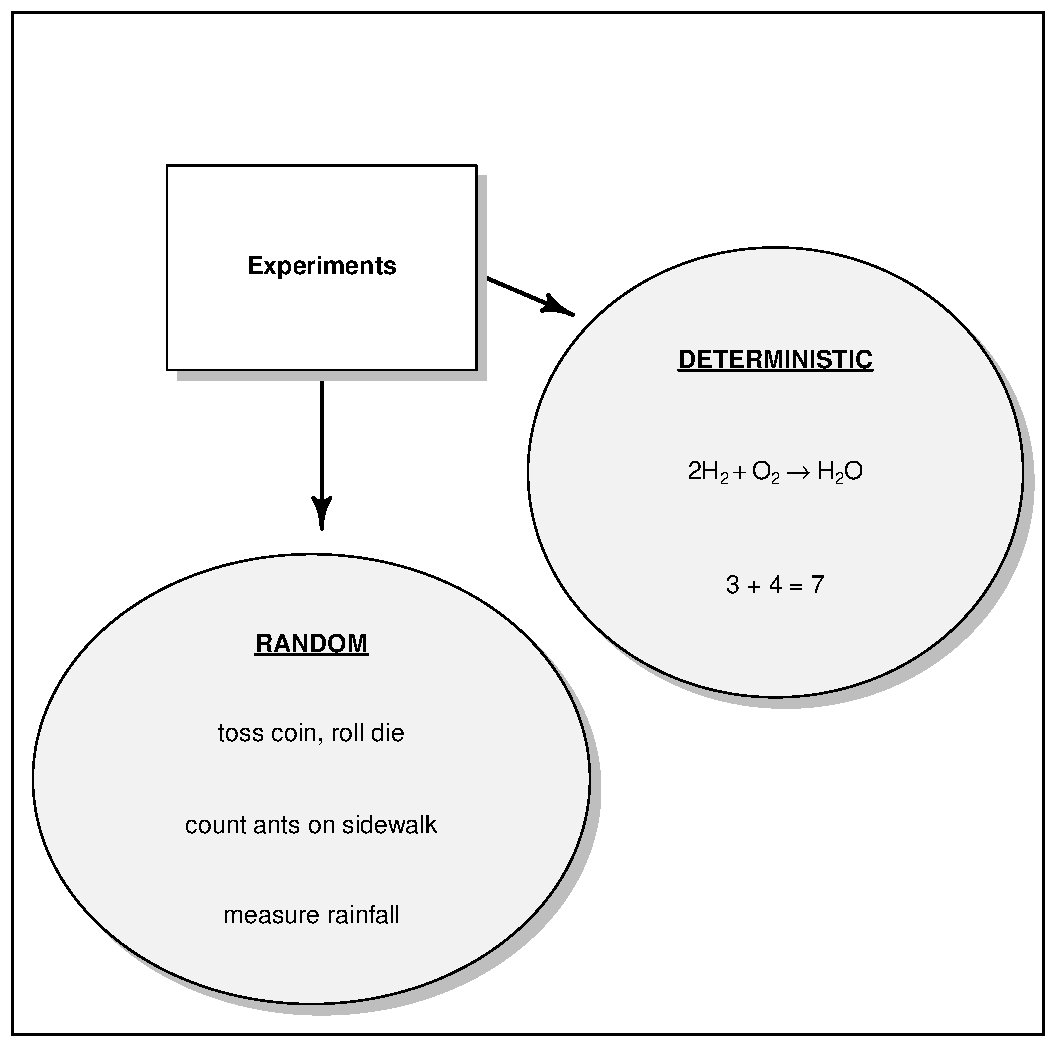
\includegraphics[width=5in, height=4in]{img/diagram.pdf}
    \caption[Two types of experiments]{Two types of experiments}
    \label{fig:diagram}
  \end{figure}
\section{Sample Spaces}
\label{sec-1-1}

\label{sec:Sample-Spaces}

For a random experiment \(E\), the set of all possible outcomes of \(E\) is called the \emph{sample space}\index{sample space} and is denoted by the letter \(S\). For a coin-toss experiment, \(S\) would be the results ``Head'' and ``Tail'', which we may represent by \( S = \{H,T \} \). Formally, the performance of a random experiment is the unpredictable selection of an outcome in \(S\).

\paragraph*{How to do it with \textsf{R}}

Most of the probability work in this book is done with the \texttt{prob} package \cite{Kernsprob}. A sample space is (usually) represented by a \emph{data frame}, that is, a rectangular collection of variables (see Section \ref{sub:Multivariate-Data}). Each row of the data frame corresponds to an outcome of the experiment. The data frame choice is convenient both for its simplicity and its compatibility with the \textsf{R} Commander. Data frames alone are, however, not sufficient to describe some of the more interesting probabilistic applications we will study later; to handle those we will need to consider a more general \emph{list} data structure. See Section \ref{sub:howto-ps-objects} for details.

\begin{example}
Consider the random experiment of dropping a Styrofoam cup onto the floor from a height of four feet. The cup hits the ground and eventually comes to rest. It could land upside down, right side up, or it could land on its side. We represent these possible outcomes of the random experiment by the following.


\begin{verbatim}
S <- data.frame(lands = c("down","up","side"))
S
\end{verbatim}

\begin{verbatim}
   lands
 1  down
 2    up
 3  side
\end{verbatim}


The sample space \texttt{S} contains the column \texttt{lands} which stores the outcomes \texttt{down}, \texttt{up}, and \texttt{side}. 

\end{example}

Some sample spaces are so common that convenience wrappers were written to set them up with minimal effort. The underlying machinery that does the work includes the \texttt{expand.grid} function in the \texttt{base} package, \texttt{combn} in the \texttt{combinat} package \cite{combinat}, and \texttt{permsn} in the \texttt{prob} package
\footnote{The seasoned \textsf{R} user can get the job done without the convenience wrappers. I encourage the beginner to use them to get started, but I also recommend that introductory students wean themselves as soon as possible. The wrappers were designed for ease and intuitive use, not for speed or efficiency.}.
Consider the random experiment of tossing a coin. The outcomes are \(H\) and \(T\). We can set up the sample space quickly with the \texttt{tosscoin} function:


\begin{verbatim}
library(prob)
tosscoin(1)
\end{verbatim}

\begin{verbatim}
   toss1
 1     H
 2     T
\end{verbatim}


The number \texttt{1} tells \texttt{tosscoin} that we only want to toss the coin once. We could toss it three times: 


\begin{verbatim}
tosscoin(3)
\end{verbatim}

\begin{verbatim}
   toss1 toss2 toss3
 1     H     H     H
 2     T     H     H
 3     H     T     H
 4     T     T     H
 5     H     H     T
 6     T     H     T
 7     H     T     T
 8     T     T     T
\end{verbatim}


Alternatively we could roll a fair die: 


\begin{verbatim}
rolldie(1)
\end{verbatim}

\begin{verbatim}
   X1
 1  1
 2  2
 3  3
 4  4
 5  5
 6  6
\end{verbatim}


The \texttt{rolldie} function defaults to a 6-sided die, but we can specify others with the \texttt{nsides} argument. The command \texttt{rolldie(3, nsides = 4)} would be used to roll a 4-sided die three times.

Perhaps we would like to draw one card from a standard set of playing cards (it is a long data frame):


\begin{verbatim}
head(cards())
\end{verbatim}

\begin{verbatim}
   rank suit
 1    2 Club
 2    3 Club
 3    4 Club
 4    5 Club
 5    6 Club
 6    7 Club
\end{verbatim}


The \texttt{cards} function that we just used has optional arguments \texttt{jokers} (if you would like Jokers to be in the deck) and \texttt{makespace} which we will discuss later. There is also a \texttt{roulette} function which returns the sample space associated with one spin on a roulette wheel. There are EU and USA versions available. Interested readers may contribute any other game or sample spaces that may be of general interest.
\subsection{Sampling from Urns}
\label{sec-1-1-1}

\label{sub:sampling-from-urns}

This is perhaps the most fundamental type of random experiment. We have an urn that contains a bunch of distinguishable objects (balls) inside. We shake up the urn, reach inside, grab a ball, and take a look. That's all.

But there are all sorts of variations on this theme. Maybe we would like to grab more than one ball -- say, two balls. What are all of the possible outcomes of the experiment now? It depends on how we sample. We could select a ball, take a look, put it back, and sample again. Another way would be to select a ball, take a look -- but do not put it back -- and sample again (equivalently, just reach in and grab two balls). There are certainly more possible outcomes of the experiment in the former case than in the latter. In the first (second) case we say that sampling is done \emph{with (without) replacement}.

There is more. Suppose we do not actually keep track of which ball came first. All we observe are the two balls, and we have no idea about the order in which they were selected. We call this \emph{unordered sampling} (in contrast to \emph{ordered}) because the order of the selections does not matter with respect to what we observe. We might as well have selected the balls and put them in a bag before looking.

Note that this one general class of random experiments contains as a special case all of the common elementary random experiments. Tossing a coin twice is equivalent to selecting two balls labeled \(H\) and \(T\) from an urn, with replacement. The die-roll experiment is equivalent to selecting a ball from an urn with six elements, labeled 1 through 6.

\paragraph*{How to do it with \textsf{R}} 

The \texttt{prob} package accomplishes sampling from urns with the \texttt{urnsamples}\index{urnsamples@\texttt{urnsamples}} function, which has arguments \texttt{x}, \texttt{size}, \texttt{replace}, and \texttt{ordered}. The argument \texttt{x} represents the urn from which sampling is to be done. The \texttt{size} argument tells how large the sample will be. The \texttt{ordered} and \texttt{replace} arguments are logical and specify how sampling will be performed. We will discuss each in turn.

\begin{example}\label{exa:sample-urn-two-from-three}
Let our urn simply contain three balls, labeled 1, 2, and 3, respectively. We are going to take a sample of size 2 from the urn. 

\paragraph*{Ordered, With Replacement}

If sampling is with replacement, then we can get any outcome 1, 2, or 3 on any draw. Further, by ``ordered'' we mean that we shall keep track of the order of the draws that we observe. We can accomplish this in \textsf{R} with


\begin{verbatim}
urnsamples(1:3, size = 2, replace = TRUE, ordered = TRUE)
\end{verbatim}


\begin{verbatim}
  X1 X2
1  1  1
2  2  1
3  3  1
4  1  2
5  2  2
6  3  2
7  1  3
8  2  3
9  3  3
\end{verbatim}

 

Notice that rows 2 and 4 are identical, save for the order in which the numbers are shown. Further, note that every possible pair of the numbers 1 through 3 are listed. This experiment is equivalent to rolling a 3-sided die twice, which we could have accomplished with \texttt{rolldie(2, nsides = 3)}.

\paragraph*{Ordered, Without Replacement}

Here sampling is without replacement, so we may not observe the same number twice in any row. Order is still important, however, so we expect to see the outcomes \texttt{1,2} and \texttt{2,1} somewhere in our data frame. 


\begin{verbatim}
urnsamples(1:3, size = 2, replace = FALSE, ordered = TRUE)
\end{verbatim}

\begin{verbatim}
   X1 X2
 1  1  2
 2  2  1
 3  1  3
 4  3  1
 5  2  3
 6  3  2
\end{verbatim}

This is just as we expected. Notice that there are less rows in this answer due to the more restrictive sampling procedure. If the numbers 1, 2, and 3 represented ``Fred'', ``Mary'', and ``Sue'', respectively, then this experiment would be equivalent to selecting two people of the three to serve as president and vice-president of a company, respectively, and the sample space shown above lists all possible ways that this could be done.

\paragraph*{Unordered, Without Replacement}

Again, we may not observe the same outcome twice, but in this case, we will only retain those outcomes which (when jumbled) would not duplicate earlier ones. 


\begin{verbatim}
urnsamples(1:3, size = 2, replace = FALSE, ordered = FALSE)
\end{verbatim}

\begin{verbatim}
   X1 X2
 1  1  2
 2  1  3
 3  2  3
\end{verbatim}

This experiment is equivalent to reaching in the urn, picking a pair, and looking to see what they are. This is the default setting of \texttt{urnsamples}, so we would have received the same output by simply typing \texttt{urnsamples(1:3, 2)}.

\paragraph*{Unordered, With Replacement}

The last possibility is perhaps the most interesting. We replace the balls after every draw, but we do not remember the order in which the draws came. 


\begin{verbatim}
urnsamples(1:3, size = 2, replace = TRUE, ordered = FALSE)
\end{verbatim}

\begin{verbatim}
   X1 X2
 1  1  1
 2  1  2
 3  1  3
 4  2  2
 5  2  3
 6  3  3
\end{verbatim}

We may interpret this experiment in a number of alternative ways. One way is to consider this as simply putting two 3-sided dice in a cup, shaking the cup, and looking inside -- as in a game of \emph{Liar's Dice}, for instance. Each row of the sample space is a potential pair we could observe. Another way is to view each outcome as a separate method to distribute two identical golf balls into three boxes labeled 1, 2, and 3. Regardless of the interpretation, \texttt{urnsamples} lists every possible way that the experiment can conclude.

\end{example}
Note that the urn does not need to contain numbers; we could have just as easily taken our urn to be \texttt{x = c("Red","Blue","Green")}. But, there is an \textbf{important} point to mention before proceeding. Astute readers will notice that in our example, the balls in the urn were \textit{distinguishable} in the sense that each had a unique label to distinguish it from the others in the urn. A natural question would be, ``What happens if your urn has indistinguishable elements, for example, what if \texttt{x = c("Red","Red","Blue")}?'' The answer is that \texttt{urnsamples} behaves as if each ball in the urn is distinguishable, regardless of its actual contents. We may thus imagine that while there are two red balls in the urn, the balls are such that we can tell them apart (in principle) by looking closely enough at the imperfections on their
surface.

In this way, when the \texttt{x} argument of \texttt{urnsamples} has repeated elements, the resulting sample space may appear to be \texttt{ordered = TRUE} even when, in fact, the call to the function was \texttt{urnsamples(..., ordered = FALSE)}. Similar remarks apply for the \texttt{replace} argument. 
\section{Events}
\label{sec-1-2}

\label{sec:Events}

An \emph{event}\index{event} \(A\) is merely a collection of outcomes, or in other words, a subset of the sample space
\footnote{This naive definition works for finite or countably infinite sample spaces, but is inadequate for sample spaces in general. In this book, we will not address the subtleties that arise, but will refer the interested reader to any text on advanced probability or measure theory.}.
After the performance of a random experiment \(E\) we say that the event \(A\) \emph{occurred} if the experiment's outcome belongs to \(A\). We say that a bunch of events \(A_{1}\), \(A_{2}\), \(A_{3}\), \ldots{} are \emph{mutually exclusive}\index{mutually exclusive} or \emph{disjoint} if \(A_{i}\cap A_{j}=\emptyset\) for any distinct pair \(A_{i}\neq A_{j}\). For instance, in the coin-toss experiment the events \( A = \{ \mbox{Heads} \}\) and \( B = \{ \mbox{Tails} \} \) would be mutually exclusive. Now would be a good time to review the algebra of sets in Appendix \ref{sec:The-Algebra-of}.

\paragraph*{How to do it with \textsf{R}}

Given a data frame sample/probability space \texttt{S}, we may extract rows using the \texttt{[]} operator: 


\begin{verbatim}
S <- tosscoin(2, makespace = TRUE) 
S[1:3, ]
\end{verbatim}

\begin{verbatim}
   toss1 toss2 probs
 1     H     H  0.25
 2     T     H  0.25
 3     H     T  0.25
\end{verbatim}


\begin{verbatim}
S[c(2,4), ]
\end{verbatim}

\begin{verbatim}
   toss1 toss2 probs
 2     T     H  0.25
 4     T     T  0.25
\end{verbatim}

and so forth. We may also extract rows that satisfy a logical expression using the \texttt{subset} function, for instance 


\begin{verbatim}
S <- cards()
\end{verbatim}


\begin{verbatim}
subset(S, suit == "Heart")
\end{verbatim}


\begin{verbatim}
   rank  suit
27    2 Heart
28    3 Heart
29    4 Heart
30    5 Heart
31    6 Heart
32    7 Heart
33    8 Heart
34    9 Heart
35   10 Heart
36    J Heart
37    Q Heart
38    K Heart
39    A Heart
\end{verbatim}


\begin{verbatim}
subset(S, rank %in% 7:9)
\end{verbatim}


\begin{verbatim}
   rank    suit
6     7    Club
7     8    Club
8     9    Club
19    7 Diamond
20    8 Diamond
21    9 Diamond
32    7   Heart
33    8   Heart
34    9   Heart
45    7   Spade
46    8   Spade
47    9   Spade
\end{verbatim}

We could continue indefinitely. Also note that mathematical expressions are allowed: 


\begin{verbatim}
subset(rolldie(3), X1+X2+X3 > 16)
\end{verbatim}

\begin{verbatim}
     X1 X2 X3
 180  6  6  5
 210  6  5  6
 215  5  6  6
 216  6  6  6
\end{verbatim}
\subsection{Functions for Finding Subsets}
\label{sec-1-2-1}


It does not take long before the subsets of interest become complicated to specify. Yet the main idea remains: we have a particular logical condition to apply to each row. If the row satisfies the condition, then it should be in the subset. It should not be in the subset otherwise. The ease with which the condition may be coded depends of course on the question being asked. Here are a few functions to get started.

\paragraph*{The \texttt{\%in\%} function}

The function \texttt{\%in\%} helps to learn whether each value of one vector lies somewhere inside another vector. 


\begin{verbatim}
x <- 1:10 
y <- 8:12 
y %in% x
\end{verbatim}

\begin{verbatim}
 [1]  TRUE  TRUE  TRUE FALSE FALSE
\end{verbatim}

Notice that the returned value is a vector of length 5 which tests whether each element of \texttt{y} is in \texttt{x}, in turn.

\paragraph*{The \texttt{isin} function}

It is more common to want to know whether the \emph{whole} vector \texttt{y} is in \texttt{x}. We can do this with the \texttt{isin} function. 


\begin{verbatim}
isin(x,y)
\end{verbatim}

\begin{verbatim}
 [1] FALSE
\end{verbatim}

Of course, one may ask why we did not try something like \texttt{all(y \%in\% x)}, which would give a single result, \texttt{TRUE}. The reason is that the answers are different in the case that \texttt{y} has repeated values. Compare: 


\begin{verbatim}
x <- 1:10 
y <- c(3,3,7)
\end{verbatim}


\begin{verbatim}
all(y %in% x)
isin(x,y)
\end{verbatim}

\begin{verbatim}
 [1] TRUE
 [1] FALSE
\end{verbatim}

The reason for the above is of course that \texttt{x} contains the value 3, but \texttt{x} does not have \emph{two} 3's. The difference is important when rolling multiple dice, playing cards, \emph{etc}. Note that there is an optional argument \texttt{ordered} which tests whether the elements of \texttt{y} appear in \texttt{x} in the order in which they are appear in \texttt{y}. The consequences are 


\begin{verbatim}
isin(x, c(3,4,5), ordered = TRUE) 
isin(x, c(3,5,4), ordered = TRUE)
\end{verbatim}

\begin{verbatim}
 [1] TRUE
 [1] FALSE
\end{verbatim}

The connection to probability is that have a data frame sample space and we would like to find a subset of that space. A \texttt{data.frame} method was written for \texttt{isin} that simply applies the function to each row of the data frame. We can see the method in action with the following: 


\begin{verbatim}
S <- rolldie(4) 
subset(S, isin(S, c(2,2,6), ordered = TRUE))
\end{verbatim}


\begin{verbatim}
     X1 X2 X3 X4
188   2  2  6  1
404   2  2  6  2
620   2  2  6  3
836   2  2  6  4
1052  2  2  6  5
1088  2  2  1  6
1118  2  1  2  6
1123  1  2  2  6
1124  2  2  2  6
1125  3  2  2  6
1126  4  2  2  6
1127  5  2  2  6
1128  6  2  2  6
1130  2  3  2  6
1136  2  4  2  6
1142  2  5  2  6
1148  2  6  2  6
1160  2  2  3  6
1196  2  2  4  6
1232  2  2  5  6
1268  2  2  6  6
\end{verbatim}

There are a few other functions written to find useful subsets, namely, \texttt{countrep} and \texttt{isrep}. Essentially these were written to test for (or count) a specific number of designated values in outcomes. See the documentation for details.
\subsection{Set Union, Intersection, and Difference}
\label{sec-1-2-2}


Given subsets \(A\) and \(B\), it is often useful to manipulate them in an algebraic fashion. To this end, we have three set operations at our disposal: union, intersection, and difference. Below is a table that summarizes the pertinent information about these operations.


\begin{center}
\begin{tabular}{llll}
\hline
 Name          &  Denoted                &  Defined by elements        &  Code                     \\
\hline
 Union         &  \(A\cup B\)            &  in \(A\) or \(B\) or both  &  \texttt{union(A,B)}      \\
 Intersection  &  \(A\cap B\)            &  in both \(A\) and \(B\)    &  \texttt{intersect(A,B)}  \\
 Difference    &  \(A\textbackslash B\)  &  in \(A\) but not in \(B\)  &  \texttt{setdiff(A,B)}    \\
\hline
\end{tabular}
\end{center}




Some examples follow. 


\begin{verbatim}
S <- cards() 
A <- subset(S, suit == "Heart") 
B <- subset(S, rank %in% 7:9)
\end{verbatim}

We can now do some set algebra: 


\begin{verbatim}
union(A,B)
\end{verbatim}


\begin{verbatim}
   rank    suit
6     7    Club
7     8    Club
8     9    Club
19    7 Diamond
20    8 Diamond
21    9 Diamond
27    2   Heart
28    3   Heart
29    4   Heart
30    5   Heart
31    6   Heart
32    7   Heart
33    8   Heart
34    9   Heart
35   10   Heart
36    J   Heart
37    Q   Heart
38    K   Heart
39    A   Heart
45    7   Spade
46    8   Spade
47    9   Spade
\end{verbatim}


\begin{verbatim}
intersect(A,B)
\end{verbatim}

\begin{verbatim}
    rank  suit
 32    7 Heart
 33    8 Heart
 34    9 Heart
\end{verbatim}


\begin{verbatim}
setdiff(A,B)
\end{verbatim}


\begin{verbatim}
   rank  suit
27    2 Heart
28    3 Heart
29    4 Heart
30    5 Heart
31    6 Heart
35   10 Heart
36    J Heart
37    Q Heart
38    K Heart
39    A Heart
\end{verbatim}


\begin{verbatim}
setdiff(B,A)
\end{verbatim}


\begin{verbatim}
   rank    suit
6     7    Club
7     8    Club
8     9    Club
19    7 Diamond
20    8 Diamond
21    9 Diamond
45    7   Spade
46    8   Spade
47    9   Spade
\end{verbatim}

Notice that \texttt{setdiff} is not symmetric. Further, note that we can calculate the \emph{complement} of a set \(A\), denoted \(A^{c}\) and defined to be the elements of \(S\) that are not in \(A\) simply with \texttt{setdiff(S,A)}. There have been methods written for \texttt{intersect}, \texttt{setdiff}, \texttt{subset}, and \texttt{union} in the case that the input objects are of class \texttt{ps}. See Section \ref{sub:howto-ps-objects}.

\begin{note}

When the \texttt{prob} package loads you will notice a message: ``\texttt{The following object(s) are masked from package:base: intersect, setdiff,}''. The reason for this message is that there already exist methods for the functions \texttt{intersect}, \texttt{setdiff}, \texttt{subset}, and \texttt{union} in the \texttt{base} package which ships with \textsf{R}. However, these methods were designed for when the arguments are vectors of the same mode. Since we are manipulating sample spaces which are data frames and lists, it was necessary to write methods to handle those cases as well. When the \texttt{prob} package is loaded, \textsf{R} recognizes that there are multiple versions of the same function in the search path and acts to shield the new definitions from the existing ones. But there is no cause for alarm, thankfully, because the \texttt{prob} functions have been carefully defined to match the usual \texttt{base} package definition in the case that the arguments are vectors. 

\end{note}
\section{Model Assignment}
\label{sec-1-3}

\label{sec:Interpreting-Probabilities}

Let us take a look at the coin-toss experiment more closely. What do we mean when we say ``the probability of Heads'' or write \(\P(\mbox{Heads})\)? Given a coin and an itchy thumb, how do we go about finding what \(\P(\mbox{Heads})\) should be?
\subsection{The Measure Theory Approach}
\label{sec-1-3-1}


This approach states that the way to handle \(\P(\mbox{Heads})\) is to define a mathematical function, called a \emph{probability measure}, on the sample space. Probability measures satisfy certain axioms (to be introduced later) and have special mathematical properties, so not just any mathematical function will do. But in any given physical circumstance there are typically all sorts of probability measures from which to choose, and it is left to the experimenter to make a reasonable choice -- one usually based on considerations of objectivity. For the tossing coin example, a valid probability measure assigns probability \(p\) to the event \( \{ \mbox{Heads} \} \), where \(p\) is some number \(0\leq p\leq1\). An experimenter that wishes to incorporate the symmetry of the coin would choose \(p=1/2\) to balance the likelihood of \( \{\mbox{Heads} \} \) and \( \{ \mbox{Tails} \} \).

Once the probability measure is chosen (or determined), there is not much left to do. All assignments of probability are made by the probability function, and the experimenter needs only to plug the event \(\{ \mbox{Heads} \}\) into to the probability function to find \(\P(\mbox{Heads})\). In this way, the probability of an event is simply a calculated value, nothing more, nothing less. Of course this is not the whole story; there are many theorems and consequences associated with this approach that will keep us occupied for the remainder of this book. The approach is called \emph{measure theory} because the measure (probability) of a set (event) is associated with how big it is (how likely it is to occur).

The measure theory approach is well suited for situations where there is symmetry to the experiment, such as flipping a balanced coin or spinning an arrow around a circle with well-defined pie slices. It is also handy because of its mathematical simplicity, elegance, and flexibility. There are literally volumes of information that one can prove about probability measures, and the cold rules of mathematics allow us to analyze intricate probabilistic problems with vigor. 

The large degree of flexibility is also a disadvantage, however. When symmetry fails it is not always obvious what an ``objective'' choice of probability measure should be; for instance, what probability should we assign to \( \{ \mbox{Heads} \} \) if we spin the coin rather than flip it? (It is not \(1/2\).) Furthermore, the mathematical rules are restrictive when we wish to incorporate subjective knowledge into the model, knowledge which changes over time and depends on the experimenter, such as personal knowledge about the properties of the specific coin being flipped, or of the person doing the flipping.

The mathematician who revolutionized this way to do probability theory was Andrey Kolmogorov, who published a landmark monograph in 1933. See \href{http://www-history.mcs.st-andrews.ac.uk/Mathematicians/Kolmogorov.html}{here} for more information.
\subsection{Relative Frequency Approach}
\label{sec-1-3-2}


This approach states that the way to determine \(\P(\mbox{Heads})\) is to flip the coin repeatedly, in exactly the same way each time. Keep a tally of the number of flips and the number of Heads observed. Then a good approximation to \(\P(\mbox{Heads})\) will be

\begin{equation} 
\P(\mbox{Heads})\approx\frac{\mbox{number of observed Heads}}{\mbox{total number of flips}}.
\end{equation}


The mathematical underpinning of this approach is the celebrated \textbf{Law of Large Numbers} which may be loosely described as follows. Let \(E\) be a random experiment in which the event \(A\) either does or does not occur. Perform the experiment repeatedly, in an identical manner, in such a way that the successive experiments do not influence each other. After each experiment, keep a running tally of whether or not the event \(A\) occurred. Let \(S_{n}\) count the number of times that \(A\) occurred in the \(n\) experiments. Then the law of large numbers says that 

\begin{equation}
\frac{S_{n}}{n}\to\P(A)\mbox{ as }n\to\infty.
\end{equation}


As the reasoning goes, to learn about the probability of an event \(A\) we need only repeat the random experiment to get a reasonable estimate of the probability's value, and if we are not satisfied with our estimate then we may simply repeat the experiment more times all the while confident that with more and more experiments our estimate will stabilize to the true value. 

The frequentist approach is good because it is relatively light on assumptions and does not worry about symmetry or claims of objectivity like the measure-theoretic approach does. It is perfect for the spinning coin experiment. One drawback to the method is that one can never know the exact value of a probability, only a long-run approximation. It also does not work well with experiments that can not be repeated indefinitely, say, the probability that it will rain today, the chances that you get will get an A in your Statistics class, or the probability that the world is destroyed by nuclear war.

This approach was espoused by Richard von Mises in the early twentieth century, and some of his main ideas were incorporated into the measure theory approach. See \href{http://www-history.mcs.st-andrews.ac.uk/Biographies/Mises.html}{here} for more.
\subsection{The Subjective Approach}
\label{sec-1-3-3}


The subjective approach interprets probability as the experimenter's \emph{degree of belief} that the event will occur. The estimate of the probability of an event is based on the totality of the individual's knowledge at the time. As new information becomes available, the estimate is modified accordingly to best reflect his/her current knowledge. The method by which the probabilities are updated is commonly done with Bayes' Rule, discussed in Section \ref{sec:Bayes'-Rule}. 

So for the coin toss example, a person may have \(\P(\mbox{Heads})=1/2\) in the absence of additional information. But perhaps the observer knows additional information about the coin or the thrower that would shift the probability in a certain direction. For instance, parlor magicians may be trained to be quite skilled at tossing coins, and some are so skilled that they may toss a fair coin and get nothing but Heads, indefinitely. I have \emph{seen} this. It was similarly claimed in \emph{Bringing Down the House} \cite{Mezrich2003} that MIT students were accomplished enough with cards to be able to cut a deck to the same location, every single time. In such cases, one clearly should use the additional information to assign \(\P(\mbox{Heads})\) away from the symmetry value of \(1/2\).

This approach works well in situations that cannot be repeated indefinitely, for example, to assign your probability that you will get an A in this class, the chances of a devastating nuclear war, or the likelihood that a cure for the common cold will be discovered.

The roots of subjective probability reach back a long time. See \href{http://en.wikipedia.org/wiki/Subjective_probability}{here} for a short discussion and links to references about the subjective approach.
\subsection{Equally Likely Model (ELM)}
\label{sec-1-3-4}


We have seen several approaches to the assignment of a probability model to a given random experiment and they are very different in their underlying interpretation. But they all cross paths when it comes to the equally likely model which assigns equal probability to all elementary outcomes of the experiment.

The ELM appears in the measure theory approach when the experiment boasts symmetry of some kind. If symmetry guarantees that all outcomes have equal ``size'', and if outcomes with equal ``size'' should get the same probability, then the ELM is a logical objective choice for the experimenter. Consider the balanced 6-sided die, the fair coin, or the dart board with equal-sized wedges.

The ELM appears in the subjective approach when the experimenter resorts to indifference or ignorance with respect to his/her knowledge of the outcome of the experiment. If the experimenter has no prior knowledge to suggest that (s)he prefer Heads over Tails, then it is reasonable for the him/her to assign equal subjective probability to both possible outcomes.

The ELM appears in the relative frequency approach as a fascinating fact of Nature: when we flip balanced coins over and over again, we observe that the proportion of times that the coin comes up Heads tends to \(1/2\). Of course if we assume that the measure theory applies then we can prove that the sample proportion must tend to 1/2 as expected, but that is putting the cart before the horse, in a manner of speaking.

The ELM is only available when there are finitely many elements in the sample space.

\paragraph*{How to do it with \textsf{R}}

In the \texttt{prob} package, a probability space is an object of outcomes \texttt{S} and a vector of probabilities (called \texttt{probs}) with entries that correspond to each outcome in \texttt{S}. When \texttt{S} is a data frame, we may simply add a column called \texttt{probs} to \texttt{S} and we will be finished; the probability space will simply be a data frame which we may call \texttt{S}. In the case that S is a list, we may combine the \texttt{outcomes} and \texttt{probs} into a larger list, \texttt{space}; it will have two components: \texttt{outcomes} and \texttt{probs}. The only requirements we need are for the entries of \texttt{probs} to be nonnegative and \texttt{sum(probs)} to be one.

To accomplish this in \textsf{R}, we may use the \texttt{probspace} function. The general syntax is \texttt{probspace(x, probs)}, where \texttt{x} is a sample space of outcomes and \texttt{probs} is a vector (of the same length as the number of outcomes in \texttt{x}). The specific choice of \texttt{probs} depends on the context of the problem, and some examples follow to demonstrate some of the more common choices. 

\begin{example}
The Equally Likely Model asserts that every outcome of the sample space has the same probability, thus, if a sample space has \(n\) outcomes, then \texttt{probs} would be a vector of length \(n\) with identical entries \(1/n\). The quickest way to generate \texttt{probs} is with the \texttt{rep} function. We will start with the experiment of rolling a die, so that \(n=6\). We will construct the sample space, generate the \texttt{probs} vector, and put them together with \texttt{probspace}. 


\begin{verbatim}
outcomes <- rolldie(1) 
p <- rep(1/6, times = 6) 
probspace(outcomes, probs = p)
\end{verbatim}

\begin{verbatim}
   X1     probs
 1  1 0.1666667
 2  2 0.1666667
 3  3 0.1666667
 4  4 0.1666667
 5  5 0.1666667
 6  6 0.1666667
\end{verbatim}

The \texttt{probspace} function is designed to save us some time in many of the most common situations. For example, due to the especial simplicity of the sample space in this case, we could have achieved the same result with only (note the name change for the first column) 


\begin{verbatim}
probspace(1:6, probs = p)
\end{verbatim}

\begin{verbatim}
   x     probs
 1 1 0.1666667
 2 2 0.1666667
 3 3 0.1666667
 4 4 0.1666667
 5 5 0.1666667
 6 6 0.1666667
\end{verbatim}

Further, since the equally likely model plays such a fundamental role in the study of probability the \texttt{probspace} function will assume that the equally model is desired if no \texttt{probs} are specified. Thus, we get the same answer with only 


\begin{verbatim}
probspace(1:6)
\end{verbatim}

\begin{verbatim}
   x     probs
 1 1 0.1666667
 2 2 0.1666667
 3 3 0.1666667
 4 4 0.1666667
 5 5 0.1666667
 6 6 0.1666667
\end{verbatim}

And finally, since rolling dice is such a common experiment in probability classes, the \texttt{rolldie} function has an additional logical argument \texttt{makespace} that will add a column of equally likely \texttt{probs} to the generated sample space: 


\begin{verbatim}
rolldie(1, makespace = TRUE)
\end{verbatim}

\begin{verbatim}
   X1     probs
 1  1 0.1666667
 2  2 0.1666667
 3  3 0.1666667
 4  4 0.1666667
 5  5 0.1666667
 6  6 0.1666667
\end{verbatim}

\noindent or just \texttt{rolldie(1, TRUE)}. Many of the other sample space functions (\texttt{tosscoin}, \texttt{cards}, \texttt{roulette}, \textit{etc}.) have similar \texttt{makespace} arguments. Check the documentation for details.

\end{example}

One sample space function that does NOT have a \texttt{makespace} option is the \texttt{urnsamples} function. This was intentional. The reason is that under the varied sampling assumptions the outcomes in the respective sample spaces are NOT, in general, equally likely. It is important for the user to carefully consider the experiment to decide whether or not the outcomes are equally likely and then use \texttt{probspace} to assign the model.

\begin{example}
\label{exa:unbalanced-coin}\textbf{An unbalanced coin.} While the \texttt{makespace} argument to \texttt{tosscoin} is useful to represent the tossing of a \emph{fair} coin, it is not always appropriate. For example, suppose our coin is not perfectly balanced, for instance, maybe the ``\(H\)'' side is somewhat heavier such that the chances of a \(H\) appearing in a single toss is 0.70 instead of 0.5. We may set up the probability space with 


\begin{verbatim}
probspace(tosscoin(1), probs = c(0.70, 0.30))
\end{verbatim}

\begin{verbatim}
   toss1 probs
 1     H   0.7
 2     T   0.3
\end{verbatim}

The same procedure can be used to represent an unbalanced die, roulette wheel, \textit{etc}.

\end{example}
\subsection{Words of Warning}
\label{sec-1-3-5}


It should be mentioned that while the splendour of \textsf{R} is uncontested,  it, like everything else, has limits both with respect to the sample/probability spaces it can manage and with respect to the finite accuracy of the representation of most numbers (see the \textsf{R} FAQ 7.31). When playing around with probability, one may be tempted to set up a probability space for tossing 100 coins or rolling 50 dice in an attempt to answer some scintillating question. (Bear in mind: rolling a die just 9 times has a sample space with over \emph{10 million} outcomes.)

Alas, even if there were enough RAM to barely hold the sample space (and there were enough time to wait for it to be generated), the infinitesimal probabilities that are associated with \emph{so many} outcomes make it difficult for the underlying machinery to handle reliably. In some cases, special algorithms need to be called just to give something
that holds asymptotically. User beware.
\section{Properties of Probability}
\label{sec-1-4}

\label{sec:Properties-of-Probability}
\subsection{Probability Functions}
\label{sec-1-4-1}

\label{sub:Probability-Functions}

A \emph{probability function} is a rule that associates with each event \(A\) of the sample space a unique number \(\P(A)=p\), called the \emph{probability of} \(A\). Any probability function \(\P\) satisfies the following three Kolmogorov Axioms: 

\begin{ax}
\label{ax:prob-nonnegative}\(\P(A)\geq0\) for any event \(A\subset S\).
\end{ax}

\begin{ax}
\label{ax:total-mass-one}\(\P(S)=1\).
\end{ax}

\begin{ax}
\label{ax:countable-additivity}If the events \(A_{1}\), \(A_{2}\),
\(A_{3}\)... are disjoint then

\begin{equation}
\P\left(\bigcup_{i=1}^{n}A_{i}\right)=\sum_{i=1}^{n}\P(A_{i})\mbox{ for every }n,
\end{equation}

and furthermore,

\begin{equation}
\P\left(\bigcup_{i=1}^{\infty}A_{i}\right)=\sum_{i=1}^{\infty}\P(A_{i}).
\end{equation}

\end{ax}

The intuition behind the axioms goes like this: first, the probability of an event should never be negative. Second, since the sample space contains all possible outcomes, its probability should be one, or 100\%. The last axiom may look intimidating but it simply means that in a sequence of disjoint events (in other words, sets that do not overlap), the total probability (measure) should equal the sum of its parts. For example, the chance of rolling a 1 or a 2 on a die should be the chance of rolling a 1 plus the chance of rolling a 2.
\subsection{Properties}
\label{sec-1-4-2}


For any events \(A\) and \(B\),

\begin{enumerate}
\item \(\P(A^{c})=1-\P(A)\).\label{enu:prop-prob-complement} 

  \begin{proof}
  Since \(A\cup A^{c}=S\) and \(A\cap A^{c}=\emptyset\), we have
  \[
  1=\P(S)=\P(A\cup A^{c})=\P(A)+\P(A^{c}).
  \]
  \end{proof}
\item \(\P(\emptyset)=0\).

  \begin{proof}
  Note that \(\emptyset=S^{c}\), and use Property 1.
  \end{proof}
\item If \(A\subset B\) , then \(\P(A)\leq\P(B)\).

  \begin{proof}
  Write \(B=A\cup\left(B\cap A^{c}\right)\), and notice that \(A\cap\left(B\cap A^{c}\right)=\emptyset\); thus
  \[
  \P(B)=\P(A\cup\left(B\cap A^{c}\right))=\P(A)+\P\left(B\cap A^{c}\right)\geq\P(A),
  \]
  since \(\P\left(B\cap A^{c}\right)\ge0\). 
  \end{proof}
\item \(0\leq\P(A)\leq1\).

  \begin{proof}
  The left inequality is immediate from Axiom \ref{ax:prob-nonnegative}, and the second inequality follows from Property 3 since \(A\subset S\).
  \end{proof}
\item \textbf{The General Addition Rule.}

  \begin{equation}
  \P(A\cup B)=\P(A)+\P(B)-\P(A\cap B).\label{eq:general-addition-rule-1}
  \end{equation}
  More generally, for events \(A_{1}\), \(A_{2}\), \(A_{3}\),\ldots{}, \(A_{n}\),

  \begin{equation}
  \P\left(\bigcup_{i=1}^{n}A_{i}\right)=\sum_{i=1}^{n}\P(A_{i})-\sum_{i=1}^{n-1}\sum_{j=i+1}^{n}\P(A_{i}\cap A_{j})+\cdots+(-1)^{n-1}\P\left(\bigcap_{i=1}^{n}A_{i}\right)
  \end{equation}
\item \textbf{The Theorem of Total Probability.} 

  Let \(B_{1}\), \(B_{2}\), \ldots{}, \(B_{n}\) be mutually exclusive and exhaustive. Then
  \begin{equation}
  \P(A)=\P(A\cap B_{1})+\P(A\cap B_{2})+\cdots+\P(A\cap B_{n}).\label{eq:theorem-total-probability}
  \end{equation}
\end{enumerate}
\subsection{Assigning Probabilities}
\label{sec-1-4-3}


A model of particular interest is the \emph{equally likely model}. The idea is to divide the sample space \(S\) into a finite collection of elementary events \( \{ a_{1},\ a_{2}, \ldots, a_{N} \} \) that are equally likely in the sense that each \(a_{i}\) has equal chances of occurring. The probability function associated with this model must satisfy \(\P(S)=1\), by Axiom 2. On the other hand, it must also satisfy
\[
\P(S)=\P( \{ a_{1},\ a_{2},\ldots,a_{N} \} )=\P(a_{1}\cup a_{2}\cup\cdots\cup a_{N})=\sum_{i=1}^{N}\P(a_{i}),
\]
by Axiom 3. Since \(\P(a_{i})\) is the same for all \(i\), each one necessarily equals \(1/N\). 

For an event \(A\subset S\), we write \(A\) as a collection of elementary outcomes: if \( A = \{ a_{i_{1}}, a_{i_{2}}, \ldots, a_{i_{k}} \} \) then \(A\) has \(k\) elements and 
\begin{align*}
\P(A) & =\P(a_{i_{1}})+\P(a_{i_{2}})+\cdots+\P(a_{i_{k}}),\\
 & =\frac{1}{N}+\frac{1}{N}+\cdots+\frac{1}{N},\\  & =\frac{k}{N}=\frac{\#(A)}{\#(S)}.
\end{align*}
In other words, under the equally likely model, the probability of an event \(A\) is determined by the number of elementary events that \(A\) contains. 

\begin{example}
Consider the random experiment \(E\) of tossing a coin. Then the sample space is \(S=\{H,T\}\), and under the equally likely model, these two outcomes have \(\P(H)=\P(T)=1/2\). This model is taken when it is reasonable to assume that the coin is fair.
\end{example}

\begin{example}
Suppose the experiment \(E\) consists of tossing a fair coin twice. The sample space may be represented by \(S=\{HH,\, HT,\, TH,\, TT\}\). Given that the coin is fair and that the coin is tossed in an independent and identical manner, it is reasonable to apply the equally likely model. 

What is \(\P(\mbox{at least 1 Head})\)? Looking at the sample space we see the elements \(HH\), \(HT\), and \(TH\) have at least one Head; thus, \(\P(\mbox{at least 1 Head})=3/4\). 

What is \(\P(\mbox{no Heads})\)? Notice that the event \(\{ \mbox{no Heads} \} = \{ \mbox{at least one Head} \} ^{c}\), which by Property \ref{enu:prop-prob-complement} means \(\P(\mbox{no Heads})=1-\P(\mbox{at least one head})=1-3/4=1/4\). It is obvious in this simple example that the only outcome with no Heads is \(TT\), however, this complementation trick can be handy in more complicated problems.
\end{example}

\begin{example}
\label{exa:three-child-family}
Imagine a three child family, each child being either Boy (\(B\)) or Girl (\(G\)). An example sequence of siblings would be \(BGB\). The sample space may be written

\[
S=\left\{ 
\begin{array}{cccc}
BBB, & BGB, & GBB, & GGB,\\
BBG, & BGG, & GBG, & GGG
\end{array}
\right\}.
\]

Note that for many reasons (for instance, it turns out that girls are slightly more likely to be born than boys), this sample space is \emph{not} equally likely. For the sake of argument, however, we will assume that the elementary outcomes each have probability \(1/8\).

What is \(\P(\mbox{exactly 2 Boys})\)? Inspecting the sample space reveals three outcomes with exactly two boys: \( \{ BBG,\, BGB,\, GBB \} \).  Therefore \(\P(\mbox{exactly 2 Boys})=3/8\). 

What is \(\P(\mbox{at most 2 Boys})\)? One way to solve the problem would be to count the outcomes that have 2 or less Boys, but a quicker way would be to recognize that the only way that the event \(\{ \mbox{at most 2 Boys} \}\) does \emph{not} occur is the event \(\{ \mbox{all Girls} \}\).

Thus
\[
\P(\mbox{at most 2 Boys})=1-\P(GGG)=1-1/8=7/8.
\]

\end{example}

\begin{example}
Consider the experiment of rolling a six-sided die, and let the outcome be the face showing up when the die comes to rest. Then \( S = \{ 1,\,2,\,3,\,4,\,5,\,6 \} \). It is usually reasonable to suppose that the die is fair, so that the six outcomes are equally likely.
\end{example}

\begin{example}
Consider a standard deck of 52 cards. These are usually labeled with the four \emph{suits}: Clubs, Diamonds, Hearts, and Spades, and the 13 \emph{ranks}: 2, 3, 4, \ldots{}, 10, Jack (J), Queen (Q), King (K), and Ace (A). Depending on the game played, the Ace may be ranked below 2 or above King. 

Let the random experiment \(E\) consist of drawing exactly one card from a well-shuffled deck, and let the outcome be the face of the card. Define the events \( A = \{ \mbox{draw an Ace} \} \) and \( B = \{ \mbox{draw a Club} \} \). Bear in mind: we are only drawing one card.

Immediately we have \(\P(A)=4/52\) since there are four Aces in the deck; similarly, there are \(13\) Clubs which implies \(\P(B)=13/52\).

What is \(\P(A\cap B)\)? We realize that there is only one card of the 52 which is an Ace and a Club at the same time, namely, the Ace of Clubs. Therefore \(\P(A\cap B)=1/52\).

To find \(\P(A\cup B)\) we may use the above with the General Addition Rule to get

\begin{eqnarray*}
\P(A\cup B) & = & \P(A)+\P(B)-\P(A\cap B),\\
 & = & 4/52+13/52-1/52,\\
 & = & 16/52.
\end{eqnarray*}

\end{example}

\begin{example}
Staying with the deck of cards, let another random experiment be the selection of a five card stud poker hand, where ``five card stud'' means that we draw exactly five cards from the deck without replacement, no more, and no less. It turns out that the sample space \(S\) is so large and complicated that we will be obliged to settle for the trivial description \( S = \{ \mbox{all possible 5 card hands} \} \) for the time being. We will have a more precise description later.

What is \(\P(\mbox{Royal Flush})\), or in other words, \(\P(\mbox{A, K, Q, J, 10 all in the same suit})\)? 

It should be clear that there are only four possible royal flushes. Thus, if we could only count the number of outcomes in \(S\) then we could simply divide four by that number and we would have our answer under the equally likely model. This is the subject of Section \ref{sec:Methods-of-Counting}.

\end{example}

\paragraph*{How to do it with \textsf{R}}

Probabilities are calculated in the \texttt{prob} package with the \texttt{prob} function.

Consider the experiment of drawing a card from a standard deck of playing cards. Let's denote the probability space associated with the experiment as \texttt{S}, and let the subsets \texttt{A} and \texttt{B} be defined by the following: 


\begin{verbatim}
S <- cards(makespace = TRUE) 
A <- subset(S, suit == "Heart") 
B <- subset(S, rank %in% 7:9)
\end{verbatim}

Now it is easy to calculate 


\begin{verbatim}
prob(A)
\end{verbatim}

\begin{verbatim}
 [1] 0.25
\end{verbatim}

Note that we can get the same answer with 


\begin{verbatim}
prob(S, suit == "Heart")
\end{verbatim}

\begin{verbatim}
 [1] 0.25
\end{verbatim}

We also find \texttt{prob(B) = 0.23} (listed here approximately, but 12/52 actually) and \texttt{prob(S) = 1}. Internally, the \texttt{prob} function operates by summing the \texttt{probs} column of its argument. It will find subsets on-the-fly if desired.

We have as yet glossed over the details. More specifically, \texttt{prob} has three arguments: \texttt{x}, which is a probability space (or a subset of one), \texttt{event}, which is a logical expression used to define a subset, and \texttt{given}, which is described in Section \ref{sec:Conditional-Probability}.

\emph{WARNING}. The \texttt{event} argument is used to define a subset of \texttt{x}, that is, the only outcomes used in the probability calculation will be those that are elements of \texttt{x} and satisfy \texttt{event} simultaneously. In other words, \texttt{prob(x, event)} calculates 

\begin{verbatim}
 prob(intersect(x, subset(x, event)))
\end{verbatim}

Consequently, \texttt{x} should be the entire probability space in the case that \texttt{event} is non-null.
\section{Counting Methods}
\label{sec-1-5}

\label{sec:Methods-of-Counting}

The equally-likely model is a convenient and popular way to analyze random experiments. And when the equally likely model applies, finding the probability of an event \(A\) amounts to nothing more than counting the number of outcomes that \(A\) contains (together with the number of events in \(S\)). Hence, to be a master of probability one must be skilled at counting outcomes in events of all kinds.

\begin{prop}
The Multiplication Principle. Suppose that an experiment is composed of two successive steps. Further suppose that the first step may be performed in \(n_{1}\) distinct ways while the second step may be performed in \(n_{2}\) distinct ways. Then the experiment may be performed in \(n_{1}n_{2}\) distinct ways.

More generally, if the experiment is composed of \(k\) successive steps which may be performed in \(n_{1}\), \(n_{2}\), \ldots{}, \(n_{k}\) distinct ways, respectively, then the experiment may be performed in \(n_{1}n_{2}\cdots n_{k}\) distinct ways.
\end{prop}

\begin{example}
We would like to order a pizza. It will be sure to have cheese (and marinara sauce), but we may elect to add one or more of the following five (5) available toppings:
\[
\mbox{pepperoni, sausage, anchovies, olives, and green peppers.}
\]
How many distinct pizzas are possible?

There are many ways to approach the problem, but the quickest avenue employs the Multiplication Principle directly. We will separate the action of ordering the pizza into a series of stages. At the first stage, we will decide whether or not to include pepperoni on the pizza (two possibilities). At the next stage, we will decide whether or not to include sausage on the pizza (again, two possibilities). We will continue in this fashion until at last we will decide whether or not to include green peppers on the pizza.

At each stage we will have had two options, or ways, to select a pizza to be made. The Multiplication Principle says that we should multiply the 2's to find the total number of possible pizzas: \(2\cdot2\cdot2\cdot2\cdot2=2^{5}=32\).

\end{example}

\begin{example}
We would like to buy a desktop computer to study statistics. We go to a website to build our computer our way. Given a line of products we have many options to customize our computer. In particular, there are 2 choices for a processor, 3 different operating systems, 4 levels of memory, 4 hard drives of differing sizes, and 10 choices for a monitor. How many possible types of computer must the company be prepared to build? \textbf{Answer:} \(2\cdot3\cdot4\cdot4\cdot10=960\)
\end{example}
\subsection{Ordered Samples}
\label{sec-1-5-1}


Imagine a bag with \(n\) distinguishable balls inside. Now shake up the bag and select \(k\) balls at random. How many possible sequences might we observe?

\begin{prop}
The number of ways in which one may select an ordered sample of \(k\) subjects from a population that has \(n\) distinguishable members is

\begin{itemize}
\item \(n^{k}\) if sampling is done with replacement,
\item \(n(n-1)(n-2)\cdots(n-k+1)\) if sampling is done without replacement.
\end{itemize}

\end{prop}

Recall from calculus the notation for \emph{factorials}: 

\begin{eqnarray*}
1! & = & 1,\\
2! & = & 2\cdot1=2,\\
3! & = & 3\cdot2\cdot1=6,\\
 & \vdots\\
n! & = & n(n-1)(n-2)\cdots3\cdot2\cdot1.
\end{eqnarray*}

\begin{fact}
The number of permutations of \(n\) elements is \(n!\).
\end{fact}

\begin{example}
Take a coin and flip it 7 times. How many sequences of Heads and Tails are possible? \textbf{Answer:} \(2^{7}=128\).
\end{example}

\begin{example}
In a class of 20 students, we randomly select a class president, a class vice-president, and a treasurer. How many ways can this be done? \textbf{Answer:} \(20\cdot19\cdot18=6840\).
\end{example}

\begin{example}
We rent five movies to watch over the span of two nights. We wish to watch 3 movies on the first night. How many distinct sequences of 3 movies could we possibly watch? \textbf{Answer:} \(5\cdot4\cdot3=60\).
\end{example}
\subsection{Unordered Samples}
\label{sec-1-5-2}


\begin{prop}
The number of ways in which one may select an unordered sample of \(k\) subjects from a population that has \(n\) distinguishable members is
\begin{itemize}
\item \((n-1+k)!/[(n-1)!k!]\) if sampling is done with replacement,
\item \(n!/[k!(n-k)!]\) if sampling is done without replacement.
\end{itemize}
\end{prop}

The quantity \(n!/[k!(n-k)!]\) is called a \emph{binomial coefficient} and plays a special role in mathematics; it is denoted
\begin{equation}
{n \choose k}=\frac{n!}{k!(n-k)!}\label{eq:binomial-coefficient}
\end{equation}
and is read ``\(n\) choose \(k\)''.

\begin{example}
You rent five movies to watch over the span of two nights, but only wish to watch 3 movies the first night. Your friend, Fred, wishes to borrow some movies to watch at his house on the first night. You owe Fred a favor, and allow him to select 2 movies from the set of 5. How many choices does Fred have? \textbf{Answer:} \({5 \choose 2}=10\).
\end{example}

\begin{example}
Place 3 six-sided dice into a cup. Next, shake the cup well and pour out the dice. How many distinct rolls are possible? \textbf{Answer:} \((6-1+3)!/[(6-1)!3!]={8 \choose 5}=56\). 
\end{example}


\paragraph*{How to do it with \textsf{R}}

The factorial \(n!\) is computed with the command \texttt{factorial(n)} and the binomial coefficient \({n \choose k}\) with the command \texttt{choose(n,k)}.

The sample spaces we have computed so far have been relatively small, and we can visually study them without much trouble. However, it is \emph{very} easy to generate sample spaces that are prohibitively large. And while \textsf{R} is wonderful and powerful and does almost everything except wash windows, even \textsf{R} has limits of which we should be mindful.

But we often do not need to actually generate the sample space; it suffices to count the number of outcomes. The \texttt{nsamp} function will calculate the number of rows in a sample space made by \texttt{urnsamples} without actually devoting the memory resources necessary to generate the space. The arguments are \texttt{n}, the number of (distinguishable) objects in the urn, \texttt{k}, the sample size, and \texttt{replace}, \texttt{ordered}, as above.


\begin{table}[htb]
\caption{Sampling \(k\) from \(n\) objects with \texttt{urnsamples}} \label{tab:Sampling-k-from-n}
\begin{center}
\begin{tabular}{lll}
                           &  \texttt{ordered = TRUE}  &  \texttt{ordered = FALSE}   \\
\hline
 \texttt{replace = TRUE}   &  \(n^{k}\)                &  \((n-1+k)! / [(n-1)!k!]\)  \\
 \texttt{replace = FALSE}  &  \( n! / (n-k)! \)        &  \( {n \choose k} \)        \\
\hline
\end{tabular}
\end{center}
\end{table}



\begin{example}
We will compute the number of outcomes for each of the four \texttt{urnsamples} examples that we saw in Example \ref{exa:sample-urn-two-from-three}. Recall that we took a sample of size two from an urn with three distinguishable elements.
\end{example}



\begin{verbatim}
nsamp(n=3, k=2, replace = TRUE, ordered = TRUE) 
nsamp(n=3, k=2, replace = FALSE, ordered = TRUE) 
nsamp(n=3, k=2, replace = FALSE, ordered = FALSE) 
nsamp(n=3, k=2, replace = TRUE, ordered = FALSE)
\end{verbatim}

\begin{verbatim}
 [1] 9
 [1] 6
 [1] 3
 [1] 6
\end{verbatim}

Compare these answers with the length of the data frames generated above.


\paragraph*{The Multiplication Principle}

A benefit of \texttt{nsamp} is that it is \emph{vectorized} so that entering vectors instead of numbers for \texttt{n}, \texttt{k}, \texttt{replace}, and \texttt{ordered} results in a vector of corresponding answers. This becomes particularly convenient for combinatorics problems.

\begin{example}
There are 11 artists who each submit a portfolio containing 7 paintings for competition in an art exhibition. Unfortunately, the gallery director only has space in the winners' section to accommodate 12 paintings in a row equally spread over three consecutive walls. The director decides to give the first, second, and third place winners each a wall to display the work of their choice. The walls boast 31 separate lighting options apiece. How many displays are possible?

\textbf{Answer:} The judges will pick 3 (ranked) winners out of 11 (with \texttt{rep = FALSE}, \texttt{ord = TRUE}). Each artist will select 4 of his/her paintings from 7 for display in a row (\texttt{rep = FALSE}, \texttt{ord = TRUE}), and lastly, each of the 3 walls has 31 lighting possibilities (\texttt{rep = TRUE}, \texttt{ord = TRUE}). These three numbers can be calculated quickly with 


\begin{verbatim}
n <- c(11,7,31) 
k <- c(3,4,3) 
r <- c(FALSE,FALSE,TRUE)
\end{verbatim}


\begin{verbatim}
x <- nsamp(n, k, rep = r, ord = TRUE)
\end{verbatim}

(Notice that \texttt{ordered} is always \texttt{TRUE}; \texttt{nsamp} will recycle \texttt{ordered} and \texttt{replace} to the appropriate length.) By the Multiplication Principle, the number of ways to complete the experiment is the product of the entries of \texttt{x}: 


\begin{verbatim}
prod(x)
\end{verbatim}

\begin{verbatim}
 [1] 24774195600
\end{verbatim}

Compare this with the some other ways to compute the same thing: 


\begin{verbatim}
(11*10*9)*(7*6*5*4)*313
\end{verbatim}

\begin{verbatim}
 [1] 260290800
\end{verbatim}

or alternatively 


\begin{verbatim}
prod(9:11)*prod(4:7)*313
\end{verbatim}

\begin{verbatim}
 [1] 260290800
\end{verbatim}

or even 


\begin{verbatim}
prod(factorial(c(11,7))/factorial(c(8,3)))*313
\end{verbatim}

\begin{verbatim}
 [1] 260290800
\end{verbatim}

\end{example}

As one can guess, in many of the standard counting problems there aren't substantial savings in the amount of typing; it is about the same using \texttt{nsamp} versus \texttt{factorial} and \texttt{choose}. But the virtue of \texttt{nsamp} lies in its collecting the relevant counting formulas in a one-stop shop. Ultimately, it is up to the user to choose the method that works best for him/herself. 

\begin{example}
\textbf{The Birthday Problem.} Suppose that there are \(n\) people together in a room. Each person announces the date of his/her birthday in turn. The question is: what is the probability of at least one match? If we let the event \(A\) represent 
\[
\{ \mbox{there is at least one match}, \}
\]
then would like to know \(\P(A)\), but as we will see, it is more convenient to calculate \(\P(A^{c})\).

For starters we will ignore leap years and assume that there are only 365 days in a year. Second, we will assume that births are equally distributed over the course of a year (which is not true due to all sorts of complications such as hospital delivery schedules). See \href{http://en.wikipedia.org/wiki/Birthday_problem}{here} for more.

Let us next think about the sample space. There are 365 possibilities for the first person's birthday, 365 possibilities for the second, and so forth. The total number of possible birthday sequences is therefore \(\#(S)=365^{n}\).

Now we will use the complementation trick we saw in Example \ref{exa:three-child-family}. We realize that the only situation in which \(A\) does \emph{not} occur is if there are \emph{no} matches among all people in the room, that is, only when everybody's birthday is different, so
\[
\P(A)=1-\P(A^{c})=1-\frac{\#(A^{c})}{\#(S)},
\]
since the outcomes are equally likely. Let us then suppose that there are no matches. The first person has one of 365 possible birthdays. The second person must not match the first, thus, the second person has only 364 available birthdays from which to choose. Similarly, the third person has only 363 possible birthdays, and so forth, until we reach the \(n^{\mathrm{th}}\) person, who has only \(365-n+1\) remaining possible days for a birthday. By the Multiplication Principle, we have \(\#(A^{c})=365\cdot364\cdots(365-n+1)\), and

\begin{equation}
\P(A)=1-\frac{365\cdot364\cdots(365-n+1)}{365^{n}}=1-\frac{364}{365}\cdot\frac{363}{365}\cdots\frac{(365-n+1)}{365}.
\end{equation}

As a surprising consequence, consider this: how many people does it take to be in the room so that the probability of at least one match is at least 0.50? Clearly, if there is only \(n=1\) person in the room then the probability of a match is zero, and when there are \(n=366\) people in the room there is a 100\% chance of a match (recall that we are ignoring leap years). So how many people does it take so that there is an equal chance of a match and no match?

When I have asked this question to students, the usual response is ``somewhere around \(n=180\) people'' in the room. The reasoning seems to be that in order to get a 50\% chance of a match, there should be 50\% of the available days to be occupied. The number of students in a typical classroom is 25, so as a companion question I ask students to estimate the probability of a match when there are \(n=25\) students in the room. Common estimates are a 1\%, or 0.5\%, or even 0.1\% chance of a match. After they have given their estimates, we go around the room and each student announces their birthday. More often than not, we observe a match in the class, to the students' disbelief.

Students are usually surprised to hear that, using the formula above, one needs only \(n=23\) students to have a greater than 50\% chance of at least one match. Figure \ref{fig:birthday} shows a graph of the birthday probabilities:
\end{example}





\begin{figure}[ht!]
    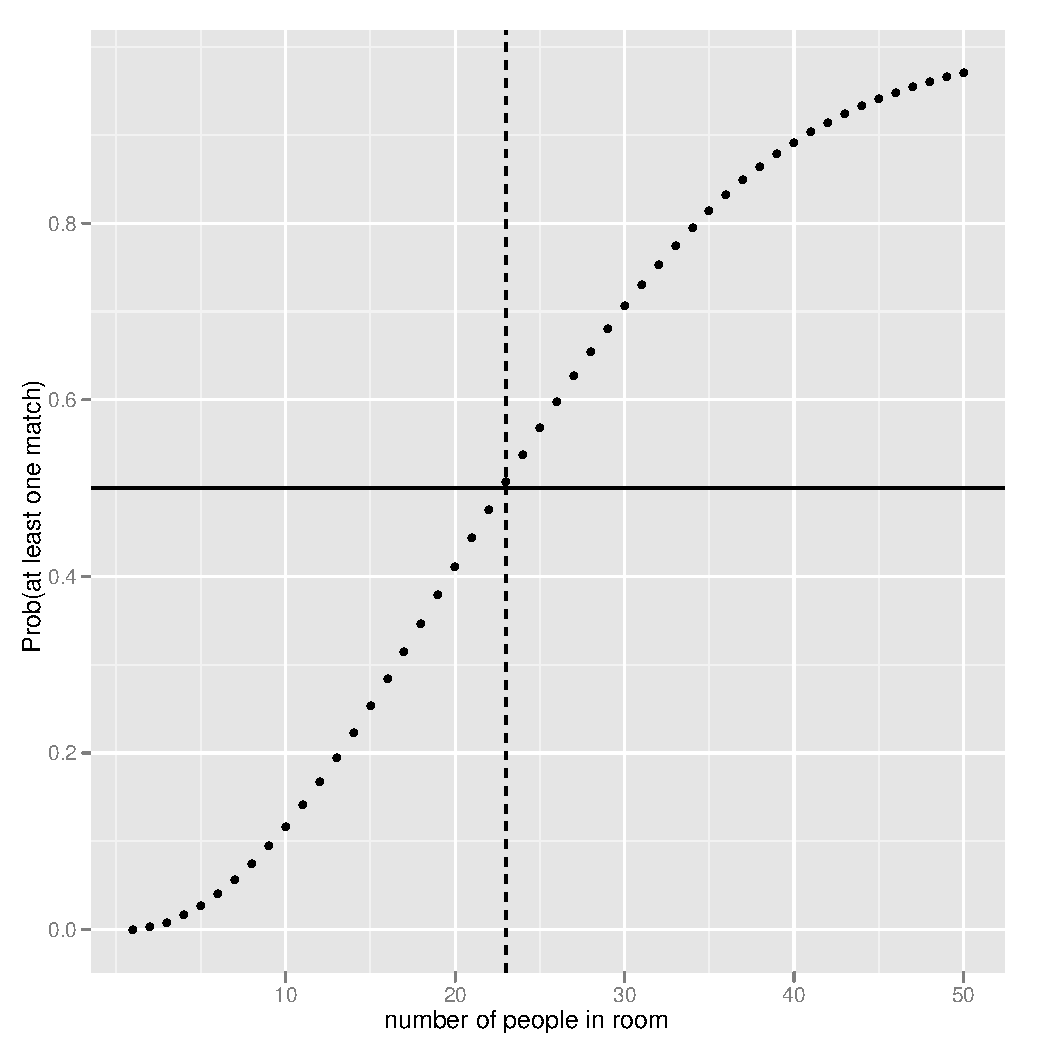
\includegraphics[width=5in, height=4in]{img/birthday.pdf}
    \caption[The birthday problem]{The birthday problem. {\small The horizontal line is at \(p=0.50\) and the vertical line is at \(n=23\).}}
    \label{fig:birthday}
  \end{figure}


\paragraph*{How to do it with \textsf{R}}

We can make the plot in Figure \ref{fig:The-Birthday-Problem} with the following sequence of commands.


\begin{verbatim}
g <- Vectorize(pbirthday.ipsur)
plot(1:50, g(1:50), xlab = "Number of people in room", 
  ylab = "Prob(at least one match)" )
abline(h = 0.5)
abline(v = 23, lty = 2)
remove(g)
\end{verbatim}

There is a \textsf{Birthday problem} item in the \textsf{Probability} menu of \texttt{RcmdrPlugin.IPSUR}. In the base \textsf{R} version, one can compute approximate probabilities for the more general case of probabilities other than 1/2, for differing total number of days in the year, and even for more than two matches.
\section{Conditional Probability}
\label{sec-1-6}

\label{sec:Conditional-Probability}

Consider a full deck of 52 standard playing cards. Now select two cards from the deck, in succession. Let \( A = \{ \mbox{first card drawn is an Ace} \} \) and \( B = \{ \mbox{second card drawn is an Ace} \} \). Since there are four Aces in the deck, it is natural to assign \( \P(A) = 4/52 \). Suppose we look at the first card. What now is the probability of \(B\)? Of course, the answer depends on the value of the first card. If the first card is an Ace, then the probability that the second also is an Ace should be \( 3/51 \), but if the first card is not an Ace, then the probability that the second is an Ace should be \( 4/51 \). As notation for these two situations we write
\[
\P(B|A)=3/51,\quad\P(B|A^{c})=4/51.
\]

\begin{defn}
The conditional probability of \(B\) given \(A\), denoted \(\P(B|A)\), is defined by
\begin{equation}
\P(B|A)=\frac{\P(A\cap B)}{\P(A)},\quad\mbox{if }\P(A)>0.
\end{equation}
We will not be discussing a conditional probability of \(B\) given \(A\) when \(\P(A)=0\), even though this theory exists, is well developed, and forms the foundation for the study of stochastic processes
\footnote{Conditional probability in this case is defined by means of \emph{conditional expectation}, a topic that is well beyond the scope of this text. The interested reader should consult an advanced text on probability theory, such as Billingsley, Resnick, or Ash Dooleans-Dade.}.
\end{defn}

\begin{example}
Toss a coin twice. The sample space is given by \(S=\{ HH,\ HT,\ TH,\ TT \} \). Let \(A= \{ \mbox{a head occurs} \} \) and \(B= \{ \mbox{a head and tail occur} \} \). It should be clear that \(\P(A)=3/4\), \(\P(B)=2/4\), and \(\P(A\cap B)=2/4\). What now are the probabilities \(\P(A|B)\) and \(\P(B|A)\)?
\[
\P(A|B)=\frac{\P(A\cap B)}{\P(B)}=\frac{2/4}{2/4}=1,
\]
in other words, once we know that a Head and Tail occur, we may be certain that a Head occurs. Next
\[
\P(B|A)=\frac{\P(A\cap B)}{\P(A)}=\frac{2/4}{3/4}=\frac{2}{3},
\]
which means that given the information that a Head has occurred, we no longer need to account for the outcome \(TT\), and the remaining three outcomes are equally likely with exactly two outcomes lying in the set \(B\). 
\end{example}

\begin{example}
\label{exa:Toss-a-six-sided-die-twice}
Toss a six-sided die twice. The sample space consists of all ordered pairs \((i,j)\) of the numbers \(1,2,\ldots,6\), that is, \( S = \{ (1,1),\ (1,2),\ldots,(6,6) \} \). We know from Section \ref{sec:Methods-of-Counting} that \( \# (S) = 6^{2} = 36 \). Let \( A = \{ \mbox{outcomes match} \} \) and \( B = \{ \mbox{sum of outcomes at least 8} \} \). The sample space may be represented by a matrix:

\begin{table}
\begin{center}
\begin{tabular}{c}
\begin{sideways}
First Roll
\end{sideways}\tabularnewline
\end{tabular}\begin{tabular}{c|cccccc|}
\multicolumn{1}{c}{} & \multicolumn{6}{c}{Second Roll}\tabularnewline
\multicolumn{1}{c}{} & 1 & 2 & 3 & 4 & 5 & \multicolumn{1}{c}{6}\tabularnewline
\cline{2-7} 
1 & \(\varprod\) &  &  &  &  & \tabularnewline
2 &  & \(\varprod\) &  &  &  & {\Large \(\bigcirc\)}\tabularnewline
3 &  &  & \(\varprod\) &  & {\Large \(\bigcirc\)} & {\Large \(\bigcirc\)}\tabularnewline
4 &  &  &  & {\huge \(\otimes\)} & {\Large \(\bigcirc\)} & {\Large \(\bigcirc\)}\tabularnewline
5 &  &  & {\Large \(\bigcirc\)} & {\Large \(\bigcirc\)} & {\huge \(\otimes\)} & {\Large \(\bigcirc\)}\tabularnewline
6 &  & {\Large \(\bigcirc\)} & {\Large \(\bigcirc\)} & {\Large \(\bigcirc\)} & {\Large \(\bigcirc\)} & {\huge \(\otimes\)}\tabularnewline
\cline{2-7} 
\end{tabular}
\caption{Rolling two dice\label{tab:Rolling-two-dice}}
\end{center}
\end{table}

The outcomes lying in the event \(A\) are marked with the symbol ``\(\varprod\)'', the outcomes falling in \(B\) are marked with ``\(\bigcirc\)'', and those in both \(A\) and \(B\) are marked ``\(\otimes\)''. Now it is clear that \(\P(A)=6/36\), \(\P(B)=15/36\), and \(\P(A\cap B)=3/36\).  Finally, 
\[
\P(A|B)=\frac{3/36}{15/36}=\frac{1}{5},\quad\P(B|A)=\frac{3/36}{6/36}=\frac{1}{2}.
\]
Again, we see that given the knowledge that \(B\) occurred (the 15 outcomes in the lower right triangle), there are 3 of the 15 that fall into the set \(A\), thus the probability is \(3/15\). Similarly, given that \(A\) occurred (we are on the diagonal), there are 3 out of 6 outcomes that also fall in \(B\), thus, the probability of \(B\) given \(A\) is 1/2. 
\end{example}

\paragraph*{How to do it with \textsf{R}}

Continuing with Example \ref{exa:Toss-a-six-sided-die-twice}, the first thing to do is set up the probability space with the \texttt{rolldie} function.


\begin{verbatim}
library(prob)
S <- rolldie(2, makespace = TRUE)  # assumes ELM
head(S)                            #  first few rows
\end{verbatim}

\begin{verbatim}
   X1 X2      probs
 1  1  1 0.02777778
 2  2  1 0.02777778
 3  3  1 0.02777778
 4  4  1 0.02777778
 5  5  1 0.02777778
 6  6  1 0.02777778
\end{verbatim}

Next we define the events


\begin{verbatim}
A <- subset(S, X1 == X2)
B <- subset(S, X1 + X2 >= 8)
\end{verbatim}

And now we are ready to calculate probabilities. To do conditional probability, we use the \texttt{given} argument of the \texttt{prob} function:


\begin{verbatim}
prob(A, given = B)
prob(B, given = A)
\end{verbatim}

\begin{verbatim}
 [1] 0.2
 [1] 0.5
\end{verbatim}

Note that we do not actually need to define the events \(A\) and \(B\) separately as long as we reference the original probability space \(S\) as the first argument of the \texttt{prob} calculation:


\begin{verbatim}
prob(S, X1==X2, given = (X1 + X2 >= 8) )
prob(S, X1+X2 >= 8, given = (X1==X2) )
\end{verbatim}

\begin{verbatim}
 [1] 0.2
 [1] 0.5
\end{verbatim}
\subsection{Properties and Rules}
\label{sec-1-6-1}


The following theorem establishes that conditional probabilities behave just like regular probabilities when the conditioned event is fixed. 

\begin{thm}
For any fixed event \(A\) with \(\P(A)>0\),
\begin{enumerate}
\item \( \P (B|A)\geq 0 \), for all events \( B \subset S\),
\item \( \P (S|A) = 1 \), and
\item If \(B_{1}\), \(B_{2}\), \(B_{3}\),\ldots{} are disjoint events, then
  \begin{equation}
  \P\left(\left.\bigcup_{k=1}^{\infty}B_{k}\:\right|A\right)=\sum_{k=1}^{\infty}\P(B_{k}|A).
  \end{equation}
\end{enumerate}
\end{thm}
In other words, \(\P(\cdot|A)\) is a legitimate probability function. With this fact in mind, the following properties are immediate:

\begin{prop}
For any events \(A\), \(B\), and \(C\) with \(\P(A)>0\),

\begin{enumerate}
\item \( \P ( B^{c} | A ) = 1 - \P (B|A).\)
\item If \(B\subset C\) then \(\P(B|A)\leq\P(C|A)\).
\item \( \P [ ( B\cup C ) | A ] = \P (B|A) + \P(C|A) - \P [ (B \cap C|A) ].\)
\item \textbf{The Multiplication Rule.} For any two events \(A\) and \(B\),
  \begin{equation}
  \P(A\cap B)=\P(A)\P(B|A).\label{eq:multiplication-rule-short}
  \end{equation}
  And more generally, for events \(A_{1}\), \(A_{2}\), \(A_{3}\),\ldots{}, \(A_{n}\),
  \begin{equation}
  \P(A_{1}\cap A_{2}\cap\cdots\cap A_{n})=\P(A_{1})\P(A_{2}|A_{1})\cdots\P(A_{n}|A_{1}\cap A_{2}\cap\cdots\cap A_{n-1}).\label{eq:multiplication-rule-long}
  \end{equation}
\end{enumerate}
\end{prop}
The Multiplication Rule is very important because it allows us to find probabilities in random experiments that have a sequential structure, as the next example shows. 

\begin{example}
\label{exa:two-cards-both-aces}
At the beginning of the section we drew two cards from a standard playing deck. Now we may answer our original question, what is \(\P(\mbox{both Aces})\)?

\[
\P(\mbox{both Aces})=\P(A\cap B)=\P(A)\P(B|A)=\frac{4}{52}\cdot\frac{3}{51}\approx0.00452.
\]

\end{example}

\paragraph*{How to do it with \textsf{R}}
\label{sub:howto-ps-objects}

Continuing Example \ref{exa:two-cards-both-aces}, we set up the probability space by way of a three step process. First we employ the \texttt{cards} function to get a data frame \texttt{L} with two columns: \texttt{rank} and \texttt{suit}. Both columns are stored internally as factors with 13 and 4 levels, respectively.

Next we sample two cards randomly from the \texttt{L} data frame by way of the \texttt{urnsamples} function. It returns a list \texttt{M} which contains all possible pairs of rows from \texttt{L} (there are \texttt{choose(52,2)} of them). The sample space for this experiment is exactly the list \texttt{M}.

At long last we associate a probability model with the sample space. This is right down the \texttt{probspace} function's alley. It assumes the equally likely model by default. We call this result \texttt{N} which is an object of class \texttt{ps} -- short for ``probability space''.

But do not be intimidated. The object \texttt{N} is nothing more than a list with two elements: \texttt{outcomes} and \texttt{probs}. The \texttt{outcomes} element is itself just another list, with \texttt{choose(52,2)} entries, each one a data frame with two rows which correspond to the pair of cards chosen. The \texttt{probs} element is just a vector with \texttt{choose(52,2)} entries all the same: \texttt{1/choose(52,2)}.

Putting all of this together we do 


\begin{verbatim}
library(prob)
L <- cards()
M <- urnsamples(L, size = 2)
N <- probspace(M)
\end{verbatim}

Now that we have the probability space \texttt{N} we are ready to do some probability. We use the \texttt{prob} function, just like before. The only trick is to specify the event of interest correctly, and recall that we were interested in \(\P(\mbox{both Aces})\). But if the cards are both Aces then the \texttt{rank} of both cards should be \texttt{A}, which sounds like a job for the \texttt{all} function:


\begin{verbatim}
prob(N, all(rank == "A"))
\end{verbatim}

\begin{verbatim}
 [1] 0.004524887
\end{verbatim}

Note that this value matches what we found in Example \ref{exa:two-cards-both-aces}, above. We could calculate all sorts of probabilities at this point; we are limited only by the complexity of the event's computer representation. 


\begin{example}
\label{exa:urn-7-red-3-green}
Consider an urn with 10 balls inside, 7 of which are red and 3 of which are green. Select 3 balls successively from the urn. Let \( A = \{ 1^{\mathrm{st}} \mbox{ ball is red} \} \), \( B = \{ 2^{\mathrm{nd}} \mbox{ ball is red} \} \), and \( C = \{ 3^{\mathrm{rd}} \mbox{ ball is red} \} \). Then

\[
\P(\mbox{all 3 balls are red})=\P(A\cap B\cap C)=\frac{7}{10}\cdot\frac{6}{9}\cdot\frac{5}{8}\approx 0.2917.
\]

\end{example}

\paragraph*{How to do it with \textsf{R}}

Example \ref{exa:urn-7-red-3-green} is similar to Example \ref{exa:two-cards-both-aces}, but it is even easier. We need to set up an urn (vector \texttt{L}) to hold the balls, we sample from \texttt{L} to get the sample space (data frame \texttt{M}), and we associate a probability vector (column \texttt{probs}) with the outcomes (rows of \texttt{M}) of the sample space. The final result is a probability space (an ordinary data frame \texttt{N}).

It is easier for us this time because our urn is a vector instead of a \texttt{cards()} data frame. Before there were two dimensions of information associated with the outcomes (rank and suit) but presently we have only one dimension (color).


\begin{verbatim}
library(prob)
L <- rep(c("red","green"), times = c(7,3))
M <- urnsamples(L, size = 3, replace = FALSE, ordered = TRUE)
N <- probspace(M)
\end{verbatim}

Now let us think about how to set up the event \(\{ \mbox{all 3 balls are red}\} \). Rows of \texttt{N} that satisfy this condition have \texttt{X1=="red" \& X2=="red" \& X3=="red"}, but there must be an easier way. Indeed, there is. The \texttt{isrep} function (short for ``is repeated'') in the \texttt{prob} package was written for this purpose. The command \texttt{isrep(N,"red",3)} will test each row of \texttt{N} to see whether the value \texttt{"red"} appears \texttt{3} times. The result is exactly what we need to define an event with the \texttt{prob} function. Observe


\begin{verbatim}
prob(N, isrep(N, "red", 3))
\end{verbatim}

\begin{verbatim}
 [1] 0.2916667
\end{verbatim}

Note that this answer matches what we found in Example \ref{exa:urn-7-red-3-green}. Now let us try some other probability questions. What is the probability of getting two =''red''=s?


\begin{verbatim}
prob(N, isrep(N, "red", 2))
\end{verbatim}

\begin{verbatim}
 [1] 0.525
\end{verbatim}


Note that the exact value is \(21/40\); we will learn a quick way to compute this in Section \ref{sec:other-discrete-distributions}. What is the probability of observing \texttt{"red"}, then \texttt{"green"}, then \texttt{"red"}?


\begin{verbatim}
prob(N, isin(N, c("red","green","red"), ordered = TRUE))
\end{verbatim}

\begin{verbatim}
 [1] 0.175
\end{verbatim}

Note that the exact value is \(7/20\) (do it with the Multiplication Rule). What is the probability of observing \texttt{"red"}, \texttt{"green"}, and \texttt{"red"}, in no particular order?


\begin{verbatim}
prob(N, isin(N, c("red","green","red")))
\end{verbatim}

\begin{verbatim}
 [1] 0.525
\end{verbatim}

We already knew this. It is the probability of observing two =''red''=s, above.


\begin{example}
Consider two urns, the first with 5 red balls and 3 green balls, and the second with 2 red balls and 6 green balls. Your friend randomly selects one ball from the first urn and transfers it to the second urn, without disclosing the color of the ball. You select one ball from the second urn. What is the probability that the selected ball is red? Let \( A = \{ \mbox{transferred ball is red} \} \) and \( B = \{ \mbox{selected ball is red} \} \). Write
\begin{align*}
B & =S\cap B\\
 & =(A\cup A^{c})\cap B\\
 & =(A\cap B)\cup(A^{c}\cap B)
\end{align*}
and notice that \(A\cap B\) and \(A^{c}\cap B\) are disjoint. Therefore
\begin{align*}
\P(B) & =\P(A\cap B)+\P(A^{c}\cap B)\\
 & =\P(A)\P(B|A)+\P(A^{c})\P(B|A^{c})\\
 & =\frac{5}{8}\cdot\frac{3}{9}+\frac{3}{8}\cdot\frac{2}{9}\\
 & =\frac{21}{72}\ 
\end{align*}
(which is 7/24 in lowest terms).

\end{example}

\begin{example}
We saw the \texttt{RcmdrTestDrive} data set in Chapter \ref{cha:introduction-to-R} in which a two-way table of the smoking status versus the gender was 


\begin{verbatim}
.Table <- xtabs( ~ smoking + gender, data = RcmdrTestDrive)
addmargins(.Table) # Table with Marginal Distributions
\end{verbatim}


If one person were selected at random from the data set, then we see from the two-way table that \(\P(\mbox{Female})=70/168\) and \(\P(\mbox{Smoker})=32/168\). Now suppose that one of the subjects quits smoking, but we do not know the person's gender. If we select one subject at random, what now is \(\P(\mbox{Female})\)? Let \( A = \{ \mbox{the quitter is a female} \} \) and \( B = \{ \mbox{selected person is a female} \} \). Write
\begin{align*}
B & =S\cap B\\
 & =(A\cup A^{c})\cap B\\
 & =(A\cap B)\cup(A^{c}\cap B)
\end{align*}
and notice that \(A\cap B\) and \(A^{c}\cap B\) are disjoint. Therefore
\begin{align*}
\P(B) & =\P(A\cap B)+\P(A^{c}\cap B),\\
 & =\P(A)\P(B|A)+\P(A^{c})\P(B|A^{c}),\\
 & =\frac{5}{8}\cdot\frac{3}{9}+\frac{3}{8}\cdot\frac{2}{9},\\
 & =\frac{21}{72},
\end{align*}
(which is 7/24 in lowest terms).

\end{example}
Using the same reasoning, we can return to the example from the beginning of the section and show that
\[
\P(\{ \mbox{second card is an Ace} \} )=4/52.
\]
 
\section{Independent Events}
\label{sec-1-7}

\label{sec:Independent-Events}

Toss a coin twice. The sample space is \(S= \{ HH,\ HT,\ TH,\ TT \} \). We know that \(\P(1^{\mathrm{st}}\mbox{ toss is }H)=2/4\), \(\P(2^{\mathrm{nd}}\mbox{ toss is }H)=2/4\), and \(\P(\mbox{both }H)=1/4\). Then
\begin{align*} \P(2^{\mathrm{nd}}\mbox{ toss is }H\ |\ 1^{\mathrm{st}}\mbox{ toss is }H) & =\frac{\P(\mbox{both }H)}{\P(1^{\mathrm{st}}\mbox{ toss is }H)},\\
 & =\frac{1/4}{2/4},\\
 & =\P(2^{\mathrm{nd}}\mbox{ toss is }H).
\end{align*}
Intuitively, this means that the information that the first toss is \(H\) has no bearing on the probability that the second toss is \(H\). The coin does not remember the result of the first toss. 

\begin{defn}
Events \(A\) and \(B\) are said to be \emph{independent} if 
\begin{equation}
\P(A\cap B)=\P(A)\P(B).
\end{equation}
Otherwise, the events are said to be \emph{dependent}. 
\end{defn}

The connection with the above example stems from the following. We know from Section \ref{sec:Conditional-Probability} that when \(\P(B)>0\) we may write
\begin{equation}
\P(A|B)=\frac{\P(A\cap B)}{\P(B)}.
\end{equation}
In the case that \(A\) and \(B\) are independent, the numerator of the fraction factors so that \(\P(B)\) cancels with the result:
\begin{equation}
\P(A|B)=\P(A)\mbox{ when \mbox{\emph{A},\emph{ B}} are independent.}
\end{equation}
The interpretation in the case of independence is that the information that the event \(B\) occurred does not influence the probability of the event \(A\) occurring. Similarly, \(\P(B|A)=\P(B)\), and so the occurrence of the event \(A\) likewise does not affect the probability of event \(B\). It may seem more natural to define \(A\) and \(B\) to be independent when \(\P(A|B)=\P(A)\); however, the conditional probability \(\P(A|B)\) is only defined when \(\P(B)>0\). Our definition is not limited by this restriction. It can be shown that when \(\P(A),\ \P(B)>0\) the two notions of independence are equivalent.

\begin{prop}
If the events \(A\) and \(B\) are independent then
\begin{itemize}
\item \(A\) and \(B^{c}\) are independent,
\item \(A^{c}\) and \(B\) are independent,
\item \(A^{c}\) and \(B^{c}\) are independent.
\end{itemize}
\end{prop}

\begin{proof}
Suppose that \(A\) and \(B\) are independent. We will show the second one; the others are similar. We need to show that
\[
\P(A^{c}\cap B)=\P(A^{c})\P(B).
\]
To this end, note that the Multiplication Rule, Equation \ref{eq:multiplication-rule-short} implies 
\begin{eqnarray*}
\P(A^{c}\cap B) & = & \P(B)\P(A^{c}|B),\\
 & = & \P(B)[1-\P(A|B)],\\
 & = & \P(B)\P(A^{c}).
\end{eqnarray*}
\end{proof}

\begin{defn}
The events \(A\), \(B\), and \(C\) are \emph{mutually independent} if the following four conditions are met: 
\begin{eqnarray*}
\P(A\cap B) & = & \P(A)\P(B),\\
\P(A\cap C) & = & \P(A)\P(C),\\
\P(B\cap C) & = & \P(B)\P(C),
\end{eqnarray*}
and
\[
\P(A\cap B\cap C)=\P(A)\P(B)\P(C).
\]
If only the first three conditions hold then \(A\), \(B\), and \(C\) are said to be independent \emph{pairwise}. Note that pairwise independence is not the same as mutual independence when the number of events is larger than two.
\end{defn}

We can now deduce the pattern for \(n\) events, \(n>3\). The events will be mutually independent only if they satisfy the product equality pairwise, then in groups of three, in groups of four, and so forth, up to all \(n\) events at once. For \(n\) events, there will be \(2^{n}-n-1\) equations that must be satisfied (see Exercise \ref{xca:numb-cond-indep}). Although these requirements for a set of events to be mutually independent may seem stringent, the good news is that for most of the situations considered in this book the conditions will all be met (or at least we will suppose that they are).

\begin{example}
\label{exa:toss-ten-coins}
Toss ten coins. What is the probability of observing at least one Head? Answer: Let \(A_{i}= \{ \mbox{the }i^{\mathrm{th}}\mbox{ coin shows }H \} ,\ i=1,2,\ldots,10\). Supposing that we toss the coins in such a way that they do not interfere with each other, this is one of the situations where all of the \(A_{i}\) may be considered mutually independent due to the nature of the tossing. Of course, the only way that there will not be at least one Head showing is if all tosses are Tails. Therefore,
\begin{align*}
\P(\mbox{at least one }H) & =1-\P(\mbox{all }T),\\
 & =1-\P(A_{1}^{c}\cap A_{2}^{c}\cap\cdots\cap A_{10}^{c}),\\
 & =1-\P(A_{1}^{c})\P(A_{2}^{c})\cdots\P(A_{10}^{c}),\\
 & =1-\left(\frac{1}{2}\right)^{10},
\end{align*}
which is approximately \(0.9990234\).

\end{example}

\paragraph*{How to do it with \textsf{R}}

\begin{example}
Toss ten coins. What is the probability of observing at least one Head?


\begin{verbatim}
S <- tosscoin(10, makespace = TRUE)
A <- subset(S, isrep(S, vals = "T", nrep = 10))
1 - prob(A)
\end{verbatim}

\begin{verbatim}
 [1] 0.9990234
\end{verbatim}

Compare this answer to what we got in Example \ref{exa:toss-ten-coins}.

\end{example}
\subsection{Independent, Repeated Experiments}
\label{sec-1-7-1}


Generalizing from above it is common to repeat a certain experiment multiple times under identical conditions and in an independent manner. We have seen many examples of this already: tossing a coin repeatedly, rolling a die or dice, \emph{etc}.

The \texttt{iidspace} function was designed specifically for this situation. It has three arguments: \texttt{x}, which is a vector of outcomes, \texttt{ntrials}, which is an integer telling how many times to repeat the experiment, and \texttt{probs} to specify the probabilities of the outcomes of \texttt{x} in a single trial. 

\begin{example}
\textbf{An unbalanced coin} (continued, see Example \ref{exa:unbalanced-coin}). It was easy enough to set up the probability space for one unbalanced toss, however, the situation becomes more complicated when there are many tosses involved. Clearly, the outcome \(HHH\) should not have the same probability as \(TTT\), which should again not have the same probability as \(HTH\). At the same time, there is symmetry in the experiment in that the coin does not remember the face it shows from toss to toss, and it is easy enough to toss the coin in a similar way repeatedly.

We may represent tossing our unbalanced coin three times with the following: 


\begin{verbatim}
iidspace(c("H","T"), ntrials = 3, probs = c(0.7, 0.3))
\end{verbatim}

\begin{verbatim}
   X1 X2 X3 probs
 1  H  H  H 0.343
 2  T  H  H 0.147
 3  H  T  H 0.147
 4  T  T  H 0.063
 5  H  H  T 0.147
 6  T  H  T 0.063
 7  H  T  T 0.063
 8  T  T  T 0.027
\end{verbatim}

As expected, the outcome \(HHH\) has the largest probability, while \(TTT\) has the smallest. (Since the trials are independent, \(\P(HHH)=0.7^{3}\) and \(\P(TTT)=0.3^{3}\), \textit{etc}.) Note that the result of the function call is a probability space, not a sample space (which we could construct already with the \texttt{tosscoin} or \texttt{urnsamples} functions). The same procedure could be used to model an unbalanced die or any other experiment that may be represented with a vector of possible outcomes.

\end{example}

Note that \texttt{iidspace} will assume \texttt{x} has equally likely outcomes if no \texttt{probs} argument is specified. Also note that the argument \texttt{x} is a \emph{vector}, not a data frame. Something like \texttt{iidspace(tosscoin(1),...)} would give an error.
\section{Bayes' Rule}
\label{sec-1-8}

\label{sec:Bayes'-Rule}

We mentioned the subjective view of probability in Section \ref{sec:Interpreting-Probabilities}. In this section we introduce a rule that allows us to update our probabilities when new information becomes available. 

\begin{thm}
\textbf{\emph{(Bayes' Rule).}} Let \(B_{1}\), \(B_{2}\), \ldots{}, \(B_{n}\) be mutually exclusive and exhaustive and let \(A\) be an event with \(\P(A)>0\). Then 
\begin{equation}
\P(B_{k}|A)=\frac{\P(B_{k})\P(A|B_{k})}{\sum_{i=1}^{n}\P(B_{i})\P(A|B_{i})},\quad k=1,2,\ldots,n.\label{eq:bayes-rule}
\end{equation}
\end{thm}

\begin{proof}
The proof follows from looking at \(\P(B_{k}\cap A)\) in two different ways. For simplicity, suppose that \(P(B_{k})>0\) for all \(k\). Then
\[
\P(A)\P(B_{k}|A)=\P(B_{k}\cap A)=\P(B_{k})\P(A|B_{k}).
\]
Since \(\P(A)>0\) we may divide through to obtain 
\[
\P(B_{k}|A)=\frac{\P(B_{k})\P(A|B_{k})}{\P(A)}.
\]
Now remembering that \(\{ B_{k} \}\) is a partition, the Theorem of Total Probability (Equation \ref{eq:theorem-total-probability}) gives the denominator of the last expression to be
\[
\P(A)=\sum_{k=1}^{n}\P(B_{k}\cap A)=\sum_{k=1}^{n}\P(B_{k})\P(A|B_{k}).
\]
\end{proof}

What does it mean? Usually in applications we are given (or know) \emph{a priori} probabilities \(\P(B_{k})\). We go out and collect some data, which we represent by the event \(A\). We want to know: how do we \textbf{update} \(\P(B_{k})\) to \(\P(B_{k}|A)\)? The answer: Bayes' Rule.

\begin{example}
\label{exa:misfiling-assistants}
\textbf{Misfiling Assistants.} In this problem, there are three assistants working at a company: Moe, Larry, and Curly. Their primary job duty is to file paperwork in the filing cabinet when papers become available. The three assistants have different work schedules:

\begin{center}
\begin{tabular}{llll}
           &  Moe   &  Larry  &  Curly  \\
\hline
 Workload  &  60\%  &  30\%   &  10\%   \\
\end{tabular}
\end{center}


That is, Moe works 60\% of the time, Larry works 30\% of the time, and Curly does the remaining 10\%, and they file documents at approximately the same speed. Suppose a person were to select one of the documents from the cabinet at random. Let \(M\) be the event
\[
M= \{ \mbox{Moe filed the document} \}
\]
and let \(L\) and \(C\) be the events that Larry and Curly, respectively, filed the document. What are these events' respective probabilities? In the absence of additional information, reasonable prior probabilities would just be


\begin{center}
\begin{tabular}{lrrr}
                    &  Moe  &  Larry  &  Curly  \\
\hline
 Prior Probability  &  0.6  &    0.3  &    0.1  \\
\end{tabular}
\end{center}



Now, the boss comes in one day, opens up the file cabinet, and selects a file at random. The boss discovers that the file has been misplaced. The boss is so angry at the mistake that (s)he threatens to fire the one who erred. The question is: who misplaced the file?

The boss decides to use probability to decide, and walks straight to the workload schedule. (S)he reasons that, since the three employees work at the same speed, the probability that a randomly selected file would have been filed by each one would be proportional to his workload. The boss notifies \textbf{Moe} that he has until the end of the day to empty his desk.

But Moe argues in his defense that the boss has ignored additional information. Moe's likelihood of having misfiled a document is smaller than Larry's and Curly's, since he is a diligent worker who pays close attention to his work. Moe admits that he works longer than the others, but he doesn't make as many mistakes as they do. Thus, Moe recommends that -- before making a decision -- the boss should update the probability (initially based on workload alone) to incorporate the likelihood of having observed a misfiled document.

And, as it turns out, the boss has information about Moe, Larry, and Curly's filing accuracy in the past (due to historical performance evaluations). The performance information may be represented by the following table:


\begin{center}
\begin{tabular}{lrrr}
               &    Moe  &  Larry  &  Curly  \\
\hline
 Misfile Rate  &  0.003  &  0.007  &  0.010  \\
\end{tabular}
\end{center}



In other words, on the average, Moe misfiles 0.3\% of the documents he is supposed to file. Notice that Moe was correct: he is the most accurate filer, followed by Larry, and lastly Curly. If the boss were to make a decision based only on the worker's overall accuracy, then \textbf{Curly} should get the axe. But Curly hears this and interjects that he only works a short period during the day, and consequently makes mistakes only very rarely; there is only the tiniest chance that he misfiled this particular document.

The boss would like to use this updated information to update the probabilities for the three assistants, that is, (s)he wants to use the additional likelihood that the document was misfiled to update his/her beliefs about the likely culprit. Let \(A\) be the event that a document is misfiled. What the boss would like to know are the three probabilities
\[
\P(M|A),\mbox{ }\P(L|A),\mbox{ and }\P(C|A).
\]
We will show the calculation for \(\P(M|A)\), the other two cases being similar. We use Bayes' Rule in the form
\[
\P(M|A)=\frac{\P(M\cap A)}{\P(A)}.
\]
Let's try to find \(\P(M\cap A)\), which is just \(\P(M)\cdot\P(A|M)\) by the Multiplication Rule. We already know \(\P(M)=0.6\) and \(\P(A|M)\) is nothing more than Moe's misfile rate, given above to be \(\P(A|M)=0.003\). Thus, we compute
\[
\P(M\cap A)=(0.6)(0.003)=0.0018.
\]
Using the same procedure we may calculate
\[
\P(L|A)=0.0021\mbox{ and }\P(C|A)=0.0010.
\]

Now let's find the denominator, \(\P(A)\). The key here is the notion that if a file is misplaced, then either Moe or Larry or Curly must have filed it; there is no one else around to do the misfiling. Further, these possibilities are mutually exclusive. We may use the Theorem of Total Probability \ref{eq:theorem-total-probability} to write
\[ 
\P(A)=\P(A\cap M)+\P(A\cap L)+\P(A\cap C).
\]
Luckily, we have computed these above. Thus
\[
\P(A)=0.0018+0.0021+0.0010=0.0049.
\]
Therefore, Bayes' Rule yields
\[
\P(M|A)=\frac{0.0018}{0.0049}\approx0.37.
\]
This last quantity is called the posterior probability that Moe misfiled the document, since it incorporates the observed data that a randomly selected file was misplaced (which is governed by the misfile rate). We can use the same argument to calculate

\begin{center}
\begin{tabular}{llll}
                        &  Moe              &  Larry            &  Curly            \\
\hline
 Posterior Probability  &  \(\approx0.37\)  &  \(\approx0.43\)  &  \(\approx0.20\)  \\
\end{tabular}
\end{center}


The conclusion: \textbf{Larry} gets the axe. What is happening is an intricate interplay between the time on the job and the misfile rate. It is not obvious who the winner (or in this case, loser) will be, and the statistician needs to consult Bayes' Rule to determine the best course of action.
\end{example}

\begin{example}
\label{exa:misfiling-assistants-multiple}
Suppose the boss gets a change of heart and does not fire anybody. But the next day (s)he randomly selects another file and again finds it to be misplaced. To decide whom to fire now, the boss would use the same procedure, with one small change. (S)he would not use the prior probabilities 60\%, 30\%, and 10\%; those are old news. Instead, she would replace the prior probabilities with the posterior probabilities just calculated. After the math she will have new posterior probabilities, updated even more from the day before.

In this way, probabilities found by Bayes' rule are always on the cutting edge, always updated with respect to the best information available at the time.
\end{example}

\paragraph*{How to do it with \textsf{R}}

There are not any special functions for Bayes' Rule in the \texttt{prob} package, but problems like the ones above are easy enough to do by hand.

\begin{example}
\textbf{Misfiling assistants} (continued from Example \ref{exa:misfiling-assistants}). We store the prior probabilities and the likelihoods in vectors and go to town.


\begin{verbatim}
prior <- c(0.6, 0.3, 0.1)
like <- c(0.003, 0.007, 0.010)
post <- prior * like
post / sum(post)
\end{verbatim}

\begin{verbatim}
 [1] 0.3673469 0.4285714 0.2040816
\end{verbatim}

\end{example}


Compare these answers with what we got in Example \ref{exa:misfiling-assistants}. We would replace \texttt{prior} with \texttt{post} in a future calculation. We could raise \texttt{like} to a power to see how the posterior is affected by future document mistakes. (Do you see why? Think back to Section \ref{sec:Independent-Events}.)


\begin{example}
Let us incorporate the posterior probability (\texttt{post}) information from the last example and suppose that the assistants misfile seven more documents. Using Bayes' Rule, what would the new posterior probabilities be?


\begin{verbatim}
newprior <- post
post <- newprior * like^7
post / sum(post)
\end{verbatim}

\begin{verbatim}
 [1] 0.0003355044 0.1473949328 0.8522695627
\end{verbatim}

We see that the individual with the highest probability of having misfiled all eight documents given the observed data is no longer Larry, but Curly. 
\end{example}

There are two important points. First, we did not divide \texttt{post} by the sum of its entries until the very last step; we do not need to calculate it, and it will save us computing time to postpone normalization until absolutely necessary, namely, until we finally want to interpret them as probabilities.

Second, the reader might be wondering what the boss would get if (s)he skipped the intermediate step of calculating the posterior after only one misfiled document. What if she started from the \emph{original} prior, then observed eight misfiled documents, and calculated the posterior? What would she get? It must be the same answer, of course.


\begin{verbatim}
fastpost <- prior * like^8
fastpost / sum(fastpost)
\end{verbatim}

\begin{verbatim}
 [1] 0.0003355044 0.1473949328 0.8522695627
\end{verbatim}

Compare this to what we got in Example \ref{exa:misfiling-assistants-multiple}.
\section{Random Variables}
\label{sec-1-9}

\label{sec:Random-Variables}

We already know about experiments, sample spaces, and events. In this section, we are interested in a \emph{number} that is associated with the experiment. We conduct a random experiment \(E\) and after learning the outcome \(\omega\) in \(S\) we calculate a number \(X\). That is, to each outcome \(\omega\) in the sample space we associate a number \(X(\omega)=x\). 

\begin{defn}
A \emph{random variable} \(X\) is a function \(X:S\to\R\) that associates to each outcome \(\omega\in S\) exactly one number \(X(\omega)=x\). 
\end{defn}

We usually denote random variables by uppercase letters such as \(X\), \(Y\), and \(Z\), and we denote their observed values by lowercase letters \(x\), \(y\), and \(z\). Just as \(S\) is the set of all possible outcomes of \(E\), we call the set of all possible values of \(X\) the \emph{support} of \(X\) and denote it by \(S_{X}\).

\begin{example}
Let \(E\) be the experiment of flipping a coin twice. We have seen that the sample space is \( S = \{ HH,\ HT,\ TH,\ TT \} \). Now define the random variable \(X = \mbox{the number of heads}\). That is, for example, \(X(HH)=2\), while \(X(HT)=1\). We may make a table of the possibilities:


\begin{center}
\begin{tabular}{lrrrr}
 \(\omega\in S\)  &  \(HH\)  &  \(HT\)  &  \(TH\)  &  \(TT\)  \\
\hline
 \(X(\omega)=x\)  &       2  &       1  &       1  &       0  \\
\end{tabular}
\end{center}



Taking a look at the second row of the table, we see that the support of \(X\) -- the set of all numbers that \(X\) assumes -- would be \( S_{X}= \{ 0,1,2 \} \).
\end{example}

\begin{example}
Let \(E\) be the experiment of flipping a coin repeatedly until observing a Head. The sample space would be \(S= \{ H,\ TH,\ TTH,\ TTTH,\ \ldots \} \). Now define the random variable \(Y=\mbox{the number of Tails before the first head}\). Then the support of \(Y\) would be \( S_{Y}= \{ 0,1,2,\ldots \} \).
\end{example}

\begin{example}
Let \(E\) be the experiment of tossing a coin in the air, and define the random variable \( Z = \mbox{the time (in seconds) until the coin hits the ground} \). In this case, the sample space is inconvenient to describe. Yet the support of \(Z\) would be \((0,\infty)\). Of course, it is reasonable to suppose that the coin will return to Earth in a short amount of time; in practice, the set \((0,\infty)\) is admittedly too large. However, we will find that in many circumstances it is mathematically convenient to study the extended set rather than a restricted one. 
\end{example}

There are important differences between the supports of \(X\), \(Y\), and \(Z\). The support of \(X\) is a finite collection of elements that can be inspected all at once. And while the support of \(Y\) cannot be exhaustively written down, its elements can nevertheless be listed in a naturally ordered sequence. Random variables with supports similar to those of \(X\) and \(Y\) are called \emph{discrete random variables}. We study these in Chapter \ref{cha:Discrete-Distributions}.

In contrast, the support of \(Z\) is a continuous interval, containing all rational and irrational positive real numbers. For this reason
\footnote{This isn't really the reason, but it serves as an effective litmus test at the introductory level. See Billingsley or Resnick.},
random variables with supports like \(Z\) are called \emph{continuous random variables}, to be studied in Chapter \ref{cha:Continuous-Distributions}.

\paragraph*{How to do it with \textsf{R}}

The primary vessel for this task is the \texttt{addrv} function. There are two ways to use it, and we will describe both.

\paragraph*{Supply a Defining Formula}

The first method is based on the \texttt{transform} function. See \texttt{?transform}. The idea is to write a formula defining the random variable inside the function, and it will be added as a column to the data frame. As an example, let us roll a 4-sided die three times, and let us define the random variable \(U=X1-X2+X3\). 


\begin{verbatim}
S <- rolldie(3, nsides = 4, makespace = TRUE) 
S <- addrv(S, U = X1-X2+X3)
\end{verbatim}

Now let's take a look at the values of \(U\). In the interest of space, we will only reproduce the first few rows of \(S\) (there are \(4^{3}=64\) rows in total). 


\begin{verbatim}
head(S)
\end{verbatim}

\begin{verbatim}
   X1 X2 X3 U    probs
 1  1  1  1 1 0.015625
 2  2  1  1 2 0.015625
 3  3  1  1 3 0.015625
 4  4  1  1 4 0.015625
 5  1  2  1 0 0.015625
 6  2  2  1 1 0.015625
\end{verbatim}

We see from the \(U\) column it is operating just like it should. We can now answer questions like


\begin{verbatim}
prob(S, U > 6)
\end{verbatim}

\begin{verbatim}
 [1] 0.015625
\end{verbatim}

\paragraph*{Supply a Function}

Sometimes we have a function laying around that we would like to apply to some of the outcome variables, but it is unfortunately tedious to write out the formula defining what the new variable would be. The \texttt{addrv} function has an argument \texttt{FUN} specifically for this case. Its value should be a legitimate function from \textsf{R}, such as \texttt{sum}, \texttt{mean}, \texttt{median}, and so forth. Or, you can define your own function. Continuing the previous example, let's define \(V=\max(X1,X2,X3)\) and \(W=X1+X2+X3\). 


\begin{verbatim}
S <- addrv(S, FUN = max, invars = c("X1","X2","X3"), name = "V") 
S <- addrv(S, FUN = sum, invars = c("X1","X2","X3"), name = "W") 
head(S)
\end{verbatim}

\begin{verbatim}
   X1 X2 X3 U V W    probs
 1  1  1  1 1 1 3 0.015625
 2  2  1  1 2 2 4 0.015625
 3  3  1  1 3 3 5 0.015625
 4  4  1  1 4 4 6 0.015625
 5  1  2  1 0 2 4 0.015625
 6  2  2  1 1 2 5 0.015625
\end{verbatim}

Notice that \texttt{addrv} has an \texttt{invars} argument to specify exactly to which columns one would like to apply the function \texttt{FUN}. If no input variables are specified, then \texttt{addrv} will apply \texttt{FUN} to all non-=probs= columns. Further, \texttt{addrv} has an optional argument \texttt{name} to give the new variable; this can be useful when adding several random variables to a probability space (as above). If not specified, the default name is \texttt{X}.

\paragraph*{Marginal Distributions}

As we can see above, often after adding a random variable \(V\) to a probability space one will find that \(V\) has values that are repeated, so that it becomes difficult to understand what the ultimate behavior of \(V\) actually is. We can use the \texttt{marginal} function to aggregate the rows of the sample space by values of \(V\), all the while accumulating the probability associated with \(V\)'s distinct values. Continuing our example from above, suppose we would like to focus entirely on the values and probabilities of \(V=\max(X1,X2,X3)\). 


\begin{verbatim}
marginal(S, vars = "V")
\end{verbatim}

\begin{verbatim}
   V    probs
 1 1 0.015625
 2 2 0.109375
 3 3 0.296875
 4 4 0.578125
\end{verbatim}

We could save the probability space of \(V\) in a data frame and study it further, if we wish. As a final remark, we can calculate the marginal distributions of multiple variables desired using the \texttt{vars} argument. For example, suppose we would like to examine the joint distribution of \(V\) and \(W\). 


\begin{verbatim}
marginal(S, vars = c("V", "W"))
\end{verbatim}


\begin{verbatim}
   V  W    probs
1  1  3 0.015625
2  2  4 0.046875
3  2  5 0.046875
4  3  5 0.046875
5  2  6 0.015625
6  3  6 0.093750
7  4  6 0.046875
8  3  7 0.093750
9  4  7 0.093750
10 3  8 0.046875
11 4  8 0.140625
12 3  9 0.015625
13 4  9 0.140625
14 4 10 0.093750
15 4 11 0.046875
16 4 12 0.015625
\end{verbatim}

Note that the default value of \texttt{vars} is the names of all columns except \texttt{probs}. This can be useful if there are duplicated rows in the probability space.

\newpage{}
\section{Chapter Exercises}
\label{sec-1-10}


\addcontentsline{toc}{section}{Chapter Exercises}
\setcounter{thm}{0}

\begin{xca}
\label{xca:numb-cond-indep}
Prove the assertion given in the text: the number of conditions that the events \(A_{1}\), \(A_{2}\), ..., \(A_{n}\) must satisfy in order to be mutually independent is \(2^{n}-n-1\). (/Hint/: think about Pascal's triangle.)
\end{xca}

\paragraph*{Answer:}

The events must satisfy the product equalities two at a time, of which there are \({n \choose 2}\), then they must satisfy an additional \({n \choose 3}\) conditions three at a time, and so on, until they satisfy the \({n \choose n}=1\) condition including all \(n\) events. In total, there are 

\[
{n \choose 2}+{n \choose 3}+\cdots+{n \choose n}=\sum_{k=0}^{n}{n \choose k}-\left[{n \choose 0}+{n \choose 1}\right]
\]

conditions to be satisfied, but the binomial series in the expression on the right is the sum of the entries of the \(n^{\mathrm{th}}\) row of Pascal's triangle, which is \(2^{n}\).

\end{document}